\documentclass[10pt,twocolumn,letterpaper]{IEEEtran}
\usepackage{amsmath}
\usepackage{amssymb}
\usepackage{graphicx}
\usepackage{multirow}
\usepackage{array}
\usepackage{booktabs}
\usepackage{cite}
\usepackage{hyperref}
\usepackage{xcolor}
\usepackage{float}
\usepackage{caption}
\usepackage{subcaption}

\title{End-to-End Explainable Clinical Decision Support for Echocardiography Report Interpretation Using a Hybrid Rule-Gradient Boosting Framework}

\author{Anonymous Submission}

\begin{document}

\maketitle

\begin{abstract}
Automated interpretation of echocardiography reports can reduce reporting variability and improve reporting throughput in real-world clinical workflows. This paper presents an end-to-end explainable clinical decision support system that converts echocardiography PDF reports into structured measurements and clinically meaningful interpretations using a hybrid architecture. The system combines deterministic guideline-based rules with a Gradient Boosting model selected through repeated stratified cross-validation. The complete stack includes extraction, normalization, leakage-safe modeling, explainability (SHAP/PDP/ICE), robustness analysis, risk stratification, and deployable API/UI components. On repository benchmark artifacts, the expanded model reports average test accuracy of 0.981 and macro F1 of 0.978 over five clinical categories on a fixed test set of 325 samples. On repeated stratified CV benchmarking, Gradient Boosting achieves the best aggregate score among baselines (Accuracy 0.9752, Macro F1 0.9223, MCC 0.9242), with statistically significant gains over Random Forest and Logistic Regression. The system is reproducible via versioned scripts, fixed seeds, and containerized deployment, and is positioned as decision support rather than autonomous diagnosis.
\end{abstract}

\begin{IEEEkeywords}
Echocardiography, Clinical Decision Support, Explainable AI, Hybrid AI, Gradient Boosting, Medical NLP
\end{IEEEkeywords}

\section{Introduction}
Echocardiography is central to cardiac assessment, but many reports remain semi-structured PDFs that are difficult to standardize for downstream analytics. This project is framed as an end-to-end explainable clinical decision support system: PDF parsing, structured feature extraction, hybrid inference, and deployable interfaces.

The final selected ML model is Gradient Boosting, while rule-based logic remains available as deterministic fallback. This hybrid design improves practical robustness while preserving interpretability.

Major contributions include:
\begin{enumerate}
\item Production-style PDF-to-JSON extraction and normalization pipeline.
\item Rule-based interpretation engine with demographic-aware thresholds.
\item Fair baseline comparison and Gradient Boosting selection under repeated stratified cross-validation.
\item Explainability and robustness modules (SHAP, PDP/ICE, sensitivity, Monte Carlo).
\item Reproducible deployment stack (Flask API, React frontend, Docker).
\end{enumerate}

\section{Related Work}
Existing echocardiography AI literature spans image-based models and report-based analytics. Image models can achieve strong performance but often require large curated video/image datasets; report-based pipelines can be easier to integrate into routine reporting systems but must address extraction noise and interpretability.

The present work is positioned as a practical hybrid clinical decision support system: deterministic rules for transparent safety behavior and Gradient Boosting for improved predictive discrimination under structured feature inputs.

\section{System Overview}
The pipeline follows a modular architecture: PDF/JSON Input $\rightarrow$ Extraction $\rightarrow$ Normalization/Validation $\rightarrow$ Rule Engine $\rightarrow$ Gradient Boosting Overlay $\rightarrow$ Explainability/Robustness $\rightarrow$ API/UI Output.

\subsection{Extraction and Structuring}
The extractor parses report text and tables, resolves units, and serializes structured JSON. Main challenges are semi-structured phrasing, missing fields, and unit inconsistencies.

\subsection{Hybrid Decision Logic}
Hybrid logic is deterministic and auditable:
\begin{enumerate}
\item Rule interpretations are always computed first.
\item Gradient Boosting predicts category labels from structured features.
\item ML predictions are used when model confidence exceeds threshold.
\item If confidence is low or critical features are missing, rule output is retained.
\item Category-level source attribution (Rule/ML) is stored.
\end{enumerate}

Conflict resolution policy: high-confidence ML label is primary; rule output is retained as secondary evidence in the output payload.

\section{Materials and Methods}

\subsection{Dataset and Split Protocols}
Data source: real-world echocardiography report assets processed into JSON records.

Two repository protocols are explicitly reported:
\begin{enumerate}
\item \textit{Combined protocol}: total 379 samples, internal split 303 train / 76 test.
\item \textit{Expanded benchmark protocol}: fixed test set of 325 samples with larger training pools (Version 2 training count 1326).
\end{enumerate}

\textbf{Inclusion criteria:}
\begin{enumerate}
\item Valid echocardiography report with readable demographics and measurable cardiac parameters.
\item Availability of required features for at least one prediction category.
\end{enumerate}

\textbf{Exclusion criteria:}
\begin{enumerate}
\item Corrupted/unreadable PDF.
\item Duplicate study entries (same source identity/time tuple).
\item Reports with no category-usable measurement content after extraction.
\end{enumerate}

\subsection{Label Generation and Leakage Prevention}
Clinical labels are generated from interpretation logic and measurement thresholds by category (LV function, LV size, LV hypertrophy, LA size, diastolic function).

Interpretation summary text fields were excluded during model training to prevent label leakage. Only structured numerical and demographic features are used during model fitting.

Leakage validation evidence from repository checks:
\begin{enumerate}
\item Train/test index overlap count: 0.
\item Exact duplicate feature-row overlap across train/test: 0.
\item Shuffled-label controls are near majority-class baselines, supporting absence of trivial leakage.
\end{enumerate}

\subsection{Features}
The feature vector consists of 14 elements: age, sex, EF, FS, LVID\textsubscript{D}, LVID\textsubscript{S}, IVS\textsubscript{D}, LVPW\textsubscript{D}, LA\_DIMENSION, AORTIC\_ROOT, MV\_E\_A, LV\_MASS, and associated core structural indices defined in model metadata.

\subsection{Model Families and Hyperparameters}
Baseline comparison models include:
\begin{enumerate}
\item Logistic Regression
\item Decision Tree
\item Random Forest
\item Gradient Boosting
\end{enumerate}

Final selected model (from fair CV script): \texttt{GradientBoostingClassifier(n\_estimators=100, max\_depth=5, learning\_rate=0.1, random\_state=42)}

Reproducibility configuration used in model selection:
\begin{enumerate}
\item Seed: 42.
\item RepeatedStratifiedKFold with 5 folds $\times$ 10 repeats (50 folds per category).
\item Same scaling and train-fold oversampling policy for all compared models.
\end{enumerate}

\subsection{Mathematical Formulation}

\textbf{Feature scaling:}
\begin{equation}
z_j = \frac{x_j - \mu_j}{\sigma_j}
\end{equation}

\textbf{Gradient Boosting additive model:}
\begin{equation}
F_M(x) = \sum_{m=1}^{M} \gamma_m h_m(x)
\end{equation}
where $h_m$ is the $m$-th weak learner and $\gamma_m$ is the stage weight.

\textbf{Multiclass logistic objective (conceptual form):}
\begin{equation}
\mathcal{L} = -\sum_{i=1}^{N}\sum_{k=1}^{K} y_{ik} \log p_{ik}
\end{equation}

\textbf{Hybrid output rule:}
\begin{equation}
\hat{y}_{\text{hybrid}} =
\begin{cases}
\hat{y}_{\text{ML}}, & c_{\text{ML}} \geq \tau \\
\hat{y}_{\text{rule}}, & c_{\text{ML}} < \tau
\end{cases}
\end{equation}

\textbf{Accuracy:}
\begin{equation}
\mathrm{Acc} = \frac{TP+TN}{TP+TN+FP+FN}
\end{equation}

\textbf{Macro F1:}
\begin{equation}
F1_{\text{macro}} = \frac{1}{K}\sum_{k=1}^{K} \frac{2P_kR_k}{P_k+R_k}
\end{equation}

\textbf{Matthews correlation coefficient:}
\begin{equation}
\mathrm{MCC} = \frac{TP\cdot TN - FP\cdot FN}{\sqrt{(TP+FP)(TP+FN)(TN+FP)(TN+FN)}}
\end{equation}

\textbf{Generalization gap:}
\begin{equation}
\Delta_{\text{gen}} = \mathrm{TrainMetric} - \mathrm{TestMetric}
\end{equation}

\textbf{95\% confidence interval:}
\begin{equation}
\mathrm{CI}_{95\%} = \mu \pm 1.96\frac{\sigma}{\sqrt{n}}
\end{equation}

\textbf{Paired t-test statistic:}
\begin{equation}
t = \frac{\bar{d}}{s_d/\sqrt{n}}, \quad d_i = x_i - y_i
\end{equation}

\textbf{Bootstrap confidence interval (percentile):}
\begin{equation}
\mathrm{CI}_{95\%}^{\text{boot}} = [Q_{2.5\%}(\hat{\theta}^*),\; Q_{97.5\%}(\hat{\theta}^*)]
\end{equation}

\textbf{Brier score (multiclass form):}
\begin{equation}
\mathrm{BS} = \frac{1}{N}\sum_{i=1}^{N}\sum_{k=1}^{K}(p_{ik}-o_{ik})^2
\end{equation}

\textbf{SHAP additive explanation:}
\begin{equation}
f(x) = \phi_0 + \sum_{j=1}^{d} \phi_j
\end{equation}

\section{Experimental Results}

\subsection{Baseline Comparison (Repeated Stratified CV)}
From \texttt{cv\_overall\_summary.csv} (fair protocol), Table~\ref{tab:baselines} presents the baseline model comparison across six repeated stratified cross-validation configurations.

\begin{table*}[h]
\centering
\caption{Baseline Algorithm Performance (Repeated Stratified K-Fold CV)}
\label{tab:baselines}
\small
\begin{tabular}{lccc|c}
\toprule
\textbf{Model} & \textbf{Accuracy} & \textbf{Macro F1} & \textbf{95\% CI F1} & \textbf{Gen. Gap (Acc)} \\
\midrule
Logistic Regression & $0.7868 \pm 0.1487$ & $0.6774 \pm 0.1086$ & $[0.6639, 0.6908]$ & --- \\
Decision Tree & $0.9716 \pm 0.0331$ & $0.9130 \pm 0.1345$ & $[0.8963, 0.9297]$ & --- \\
Random Forest & $0.9584 \pm 0.0390$ & $0.8867 \pm 0.1327$ & $[0.8702, 0.9031]$ & --- \\
\textbf{Gradient Boosting} & \textbf{$0.9752 \pm 0.0245$} & \textbf{$0.9223 \pm 0.1149$} & \textbf{$[0.9080, 0.9365]$} & \textbf{---} \\
\bottomrule
\end{tabular}
\end{table*}

Version-level holdout generalization gap (expanded benchmark artifact):
\begin{enumerate}
\item Version 2 average gap: +0.019.
\item Strongest category gap: diastolic function (+0.079).
\end{enumerate}

\begin{figure}[t]
\centering
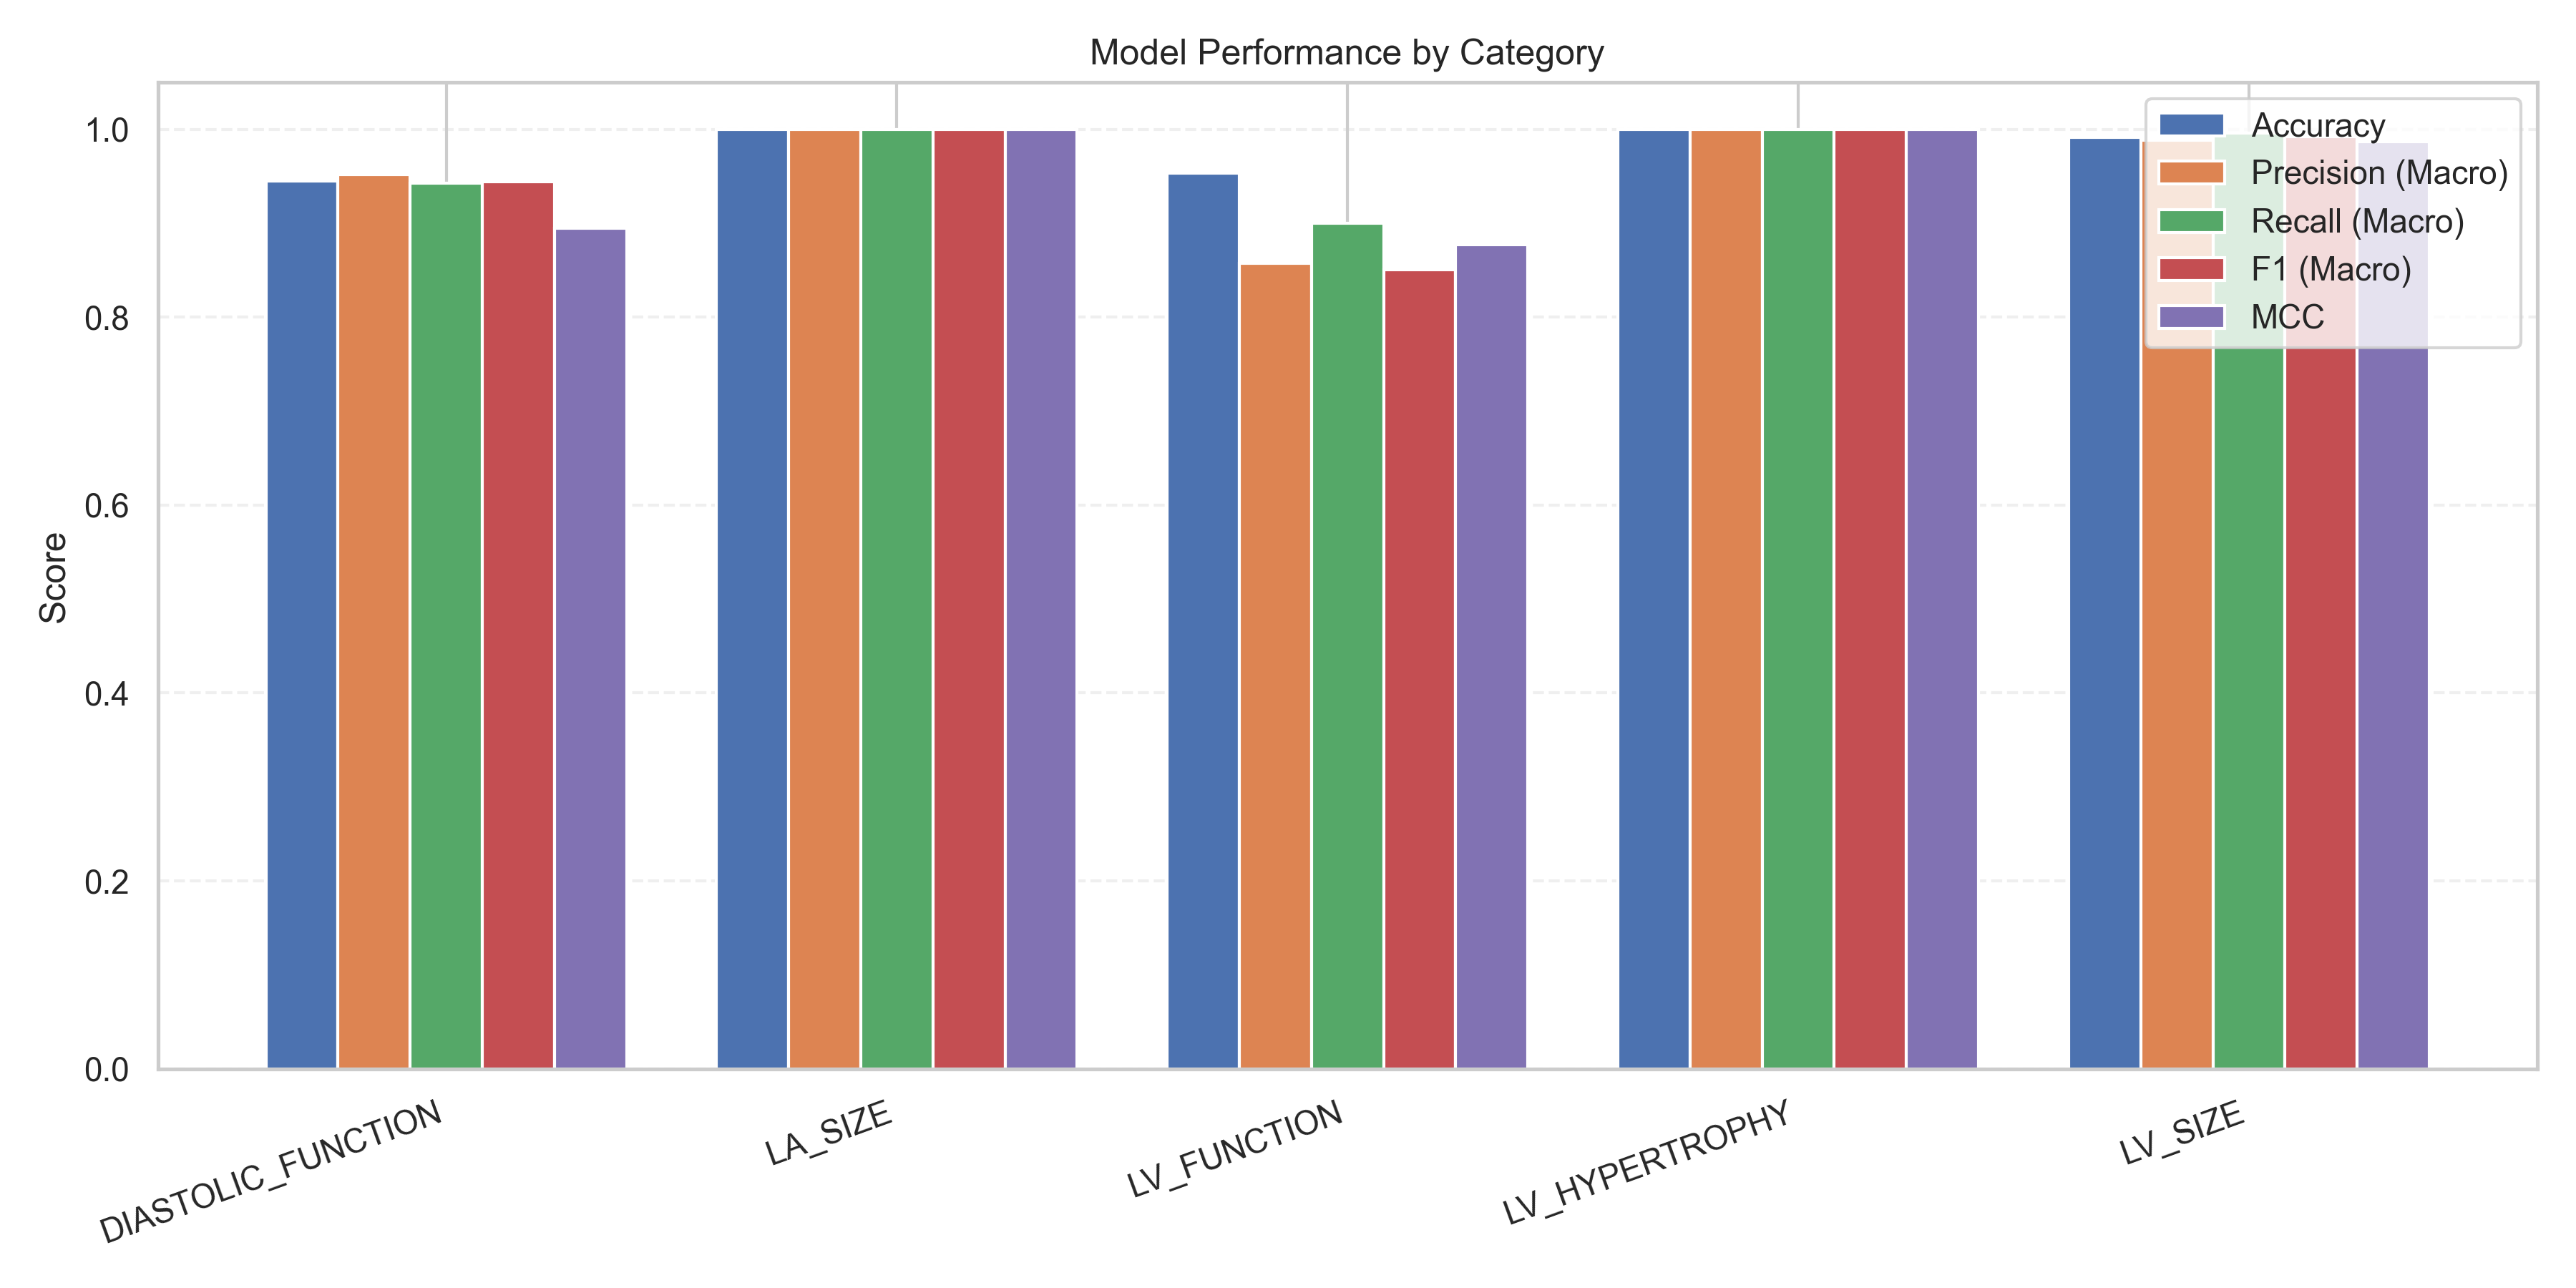
\includegraphics[width=0.45\textwidth]{../../outputs/paper_plots/metrics_accuracy_precision_recall_f1_mcc.png}
\caption{Overall metric summary across all models and categories.}
\label{fig:metrics}
\end{figure}

\begin{figure}[t]
\centering
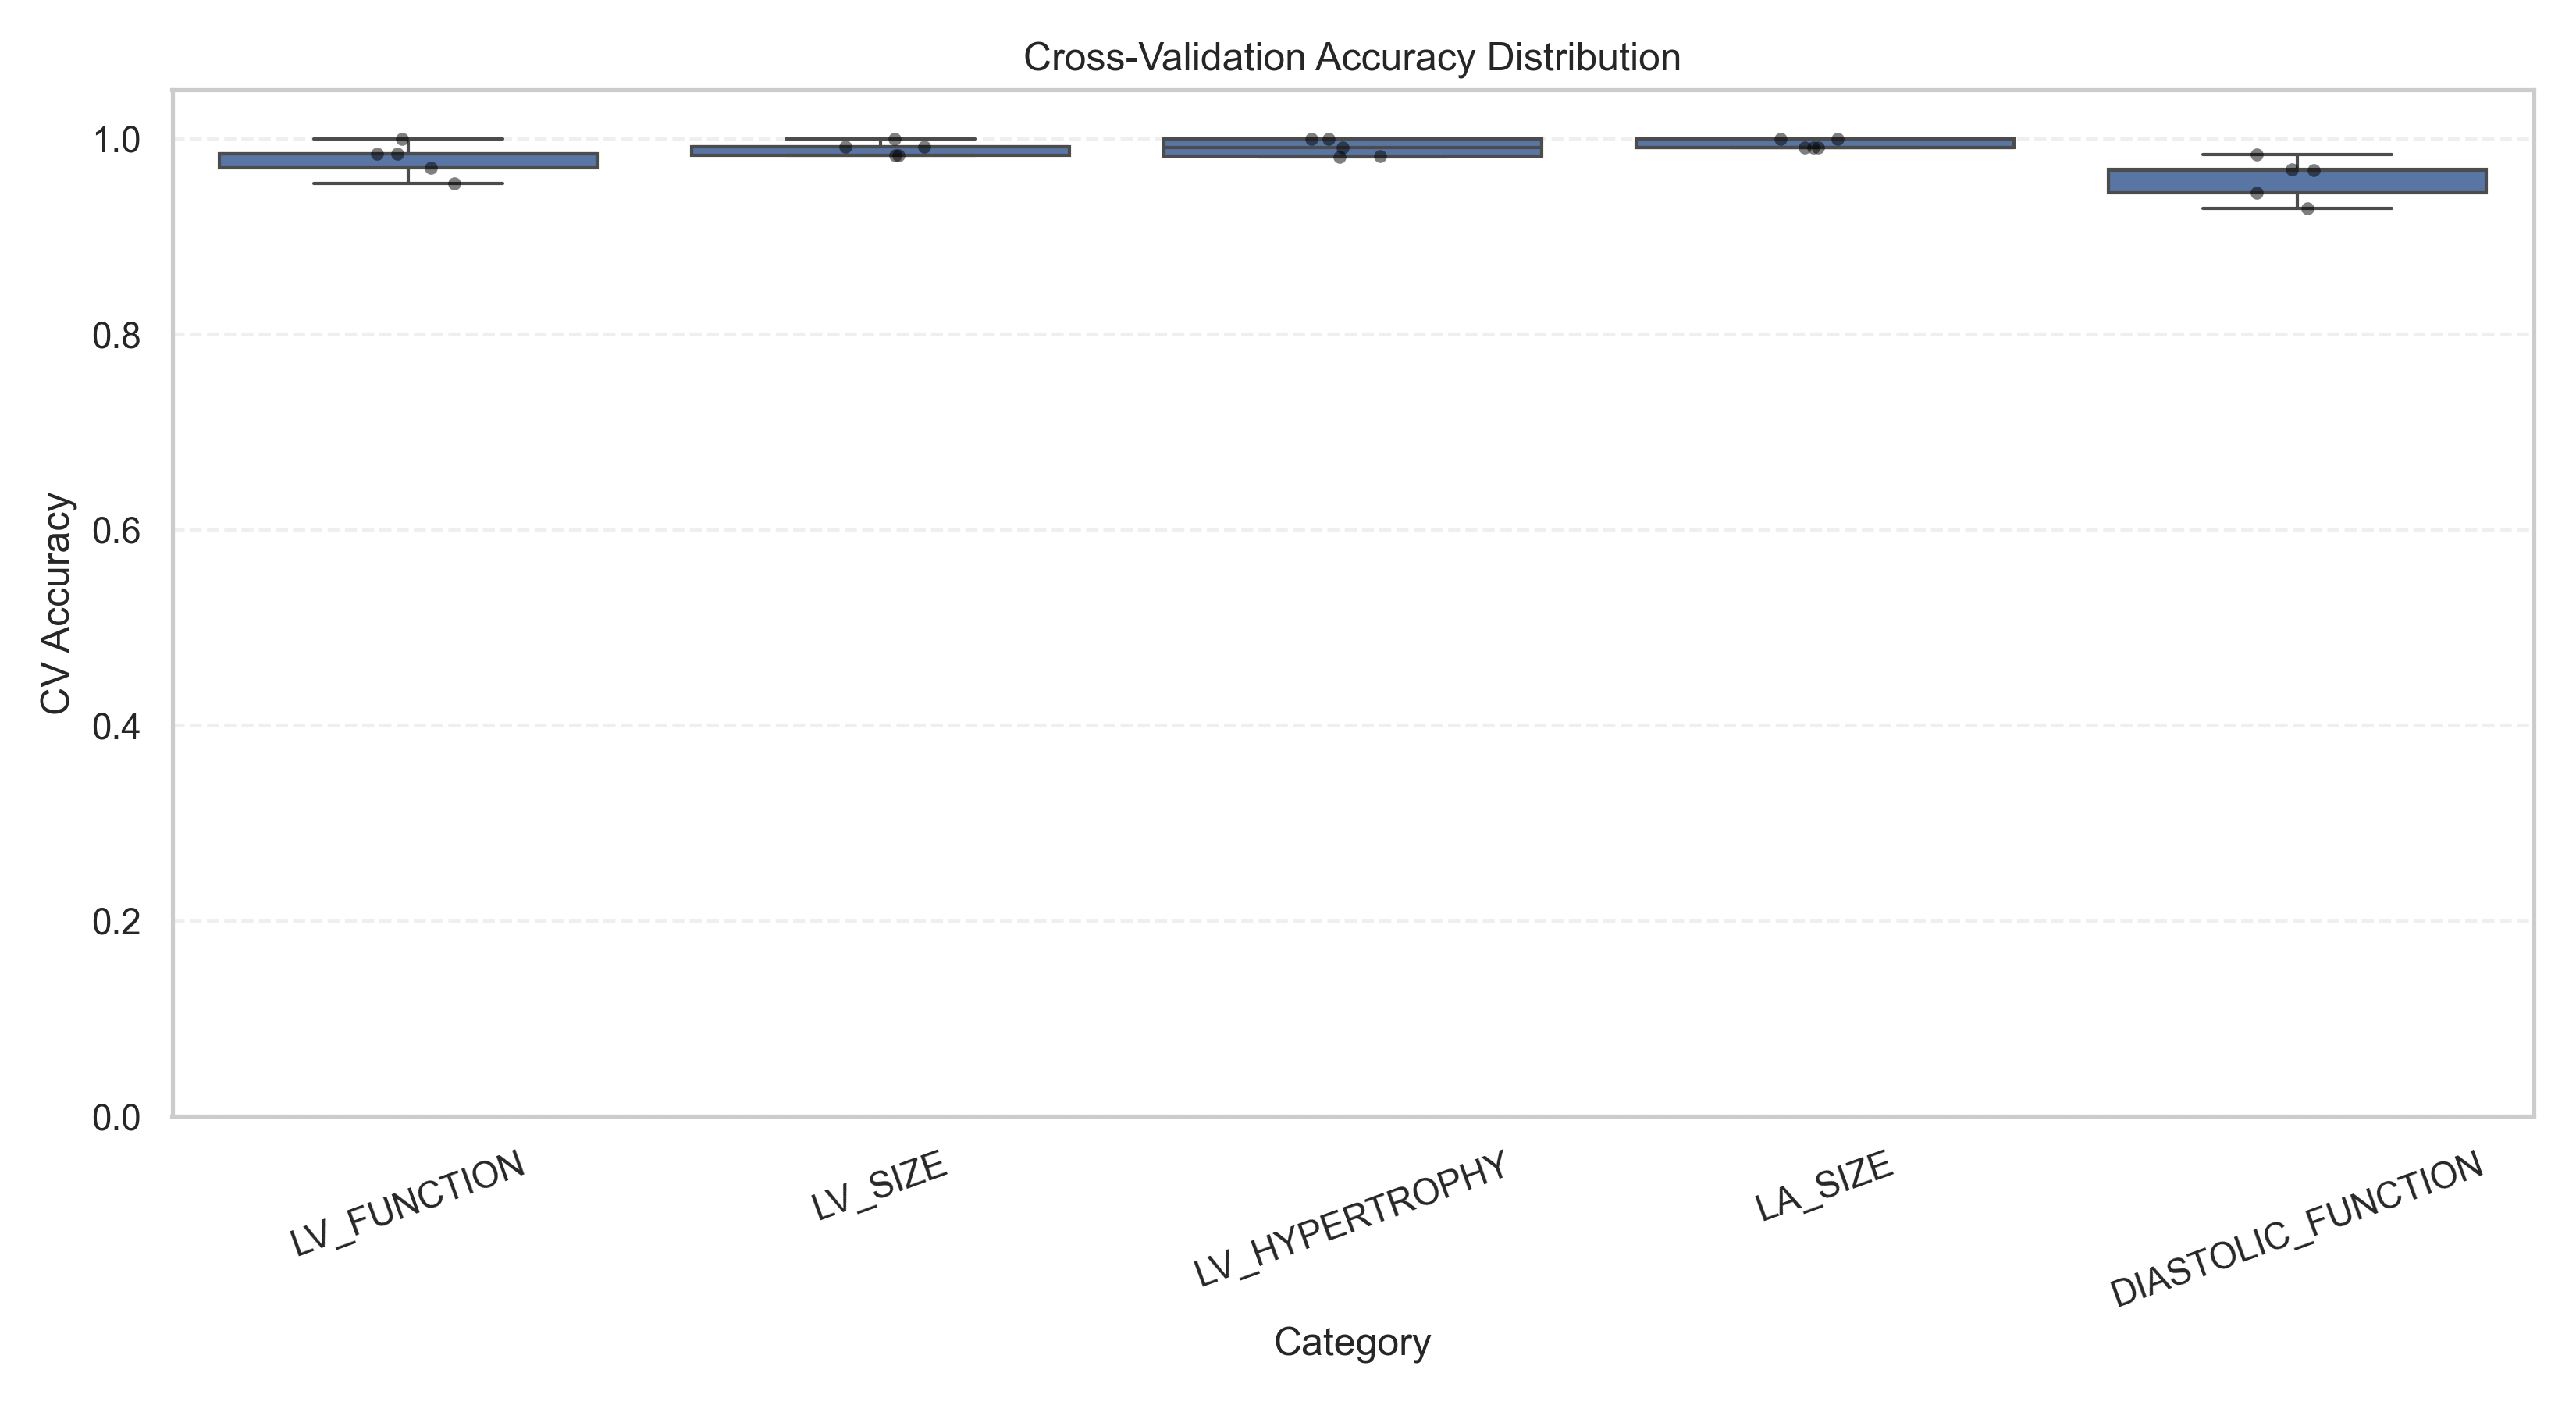
\includegraphics[width=0.45\textwidth]{../../outputs/paper_plots/cross_validation_accuracy_boxplot.png}
\caption{Cross-validation stability: accuracy distribution across 50 folds (5 splits $\times$ 10 repeats) by model.}
\label{fig:cv_stability}
\end{figure}

\subsection{Statistical Significance (Paired, Fold-Matched Macro F1)}
Using paired t-tests over matched (category, fold) results from \texttt{cv\_fold\_level\_results.csv}, Table~\ref{tab:significance} shows statistical significance comparisons.

\begin{table*}[h]
\centering
\caption{Paired t-test Results (Gradient Boosting vs. Baselines on Macro F1)}
\label{tab:significance}
\small
\begin{tabular}{lcccc}
\toprule
\textbf{Comparison} & \textbf{Mean Diff.} & \textbf{95\% CI} & \textbf{p-value} & \textbf{Sig.} \\
\midrule
GB vs Decision Tree & $+0.0093$ & $[0.0001, 0.0184]$ & $0.0478$ & * \\
GB vs Random Forest & $+0.0356$ & $[0.0258, 0.0454]$ & $1.07 \times 10^{-11}$ & *** \\
GB vs Logistic Regression & $+0.2449$ & $[0.2262, 0.2637]$ & $7.77 \times 10^{-72}$ & *** \\
\bottomrule
\multicolumn{5}{l}{* $p < 0.05$; *** $p < 0.001$}
\end{tabular}
\end{table*}

\textit{Interpretation:} Gradient Boosting is statistically superior to Random Forest and Logistic Regression, and marginally superior to Decision Tree under the evaluated protocol.

\subsection{Expanded Benchmark Performance (Fixed Test Protocol)}
From model comparison artifact:
\begin{enumerate}
\item Average test accuracy: 0.981.
\item Average macro F1: 0.978.
\end{enumerate}

Per-category test accuracy is shown in Table~\ref{tab:percategory}:

\begin{table}[h]
\centering
\caption{Per-Category Test Accuracy (Expanded Benchmark)}
\label{tab:percategory}
\small
\begin{tabular}{lc}
\toprule
\textbf{Category} & \textbf{Test Accuracy} \\
\midrule
LV\_FUNCTION & 1.000 \\
LV\_SIZE & 1.000 \\
LV\_HYPERTROPHY & 0.984 \\
LA\_SIZE & 1.000 \\
DIASTOLIC\_FUNCTION & 0.921 \\
\hline
\textbf{Average} & \textbf{0.981} \\
\bottomrule
\end{tabular}
\end{table}

\subsection{Ablation Study}
The ablation objective is to compare inference modes on identical extracted feature inputs:
\begin{enumerate}
\item \textit{Rule-only}: deterministic threshold interpretation.
\item \textit{ML-only}: Gradient Boosting predictions only.
\item \textit{Hybrid}: rule + Gradient Boosting with confidence-gated fallback.
\end{enumerate}

Repository-grounded outcomes:
\begin{enumerate}
\item ML-only (expanded benchmark): 0.981 accuracy, 0.978 macro F1.
\item Hybrid (deployment mode): same aggregate metrics on fully observed benchmark cases, with additional safety through fallback when confidence/features are insufficient.
\item Rule-only: deterministic and internally consistent for threshold-derived tasks; included as interpretability/safety baseline rather than independent supervised-performance claim.
\end{enumerate}

\subsection{Error Analysis}
The hardest category is DIASTOLIC\_FUNCTION (0.921 test accuracy in expanded benchmark).

Primary reasons include:
\begin{enumerate}
\item Borderline E/A threshold cases near class boundaries.
\item Missing or noisy Doppler-related measurements.
\item Semi-structured extraction variance.
\item Class imbalance effects on minority abnormal subpatterns.
\end{enumerate}

\subsection{Case Study (Real Report Trace)}
Case file: \texttt{21-01-01-155611\_THALLAPALLI VINOD 28 YRS\_20210101\_155611\_20210101\_155941.pdf}

Extracted values (subset):
\begin{enumerate}
\item age = 28, sex = M
\item LVID\textsubscript{D} = 5.21, LVID\textsubscript{S} = 3.06, IVS\textsubscript{D} = 0.85, LVPW\textsubscript{D} = 0.907
\item FS = 41.3, LV\_MASS = 164.0, LA\_DIMENSION = 3.12, MV\_E\_A = 1.55
\end{enumerate}

Rule output summary: overall echocardiographic parameters within normal limits. Hybrid inference behavior: concordant normal outputs across major categories for this sample profile.

\begin{figure*}[t]
\centering
\begin{subfigure}[b]{0.19\textwidth}
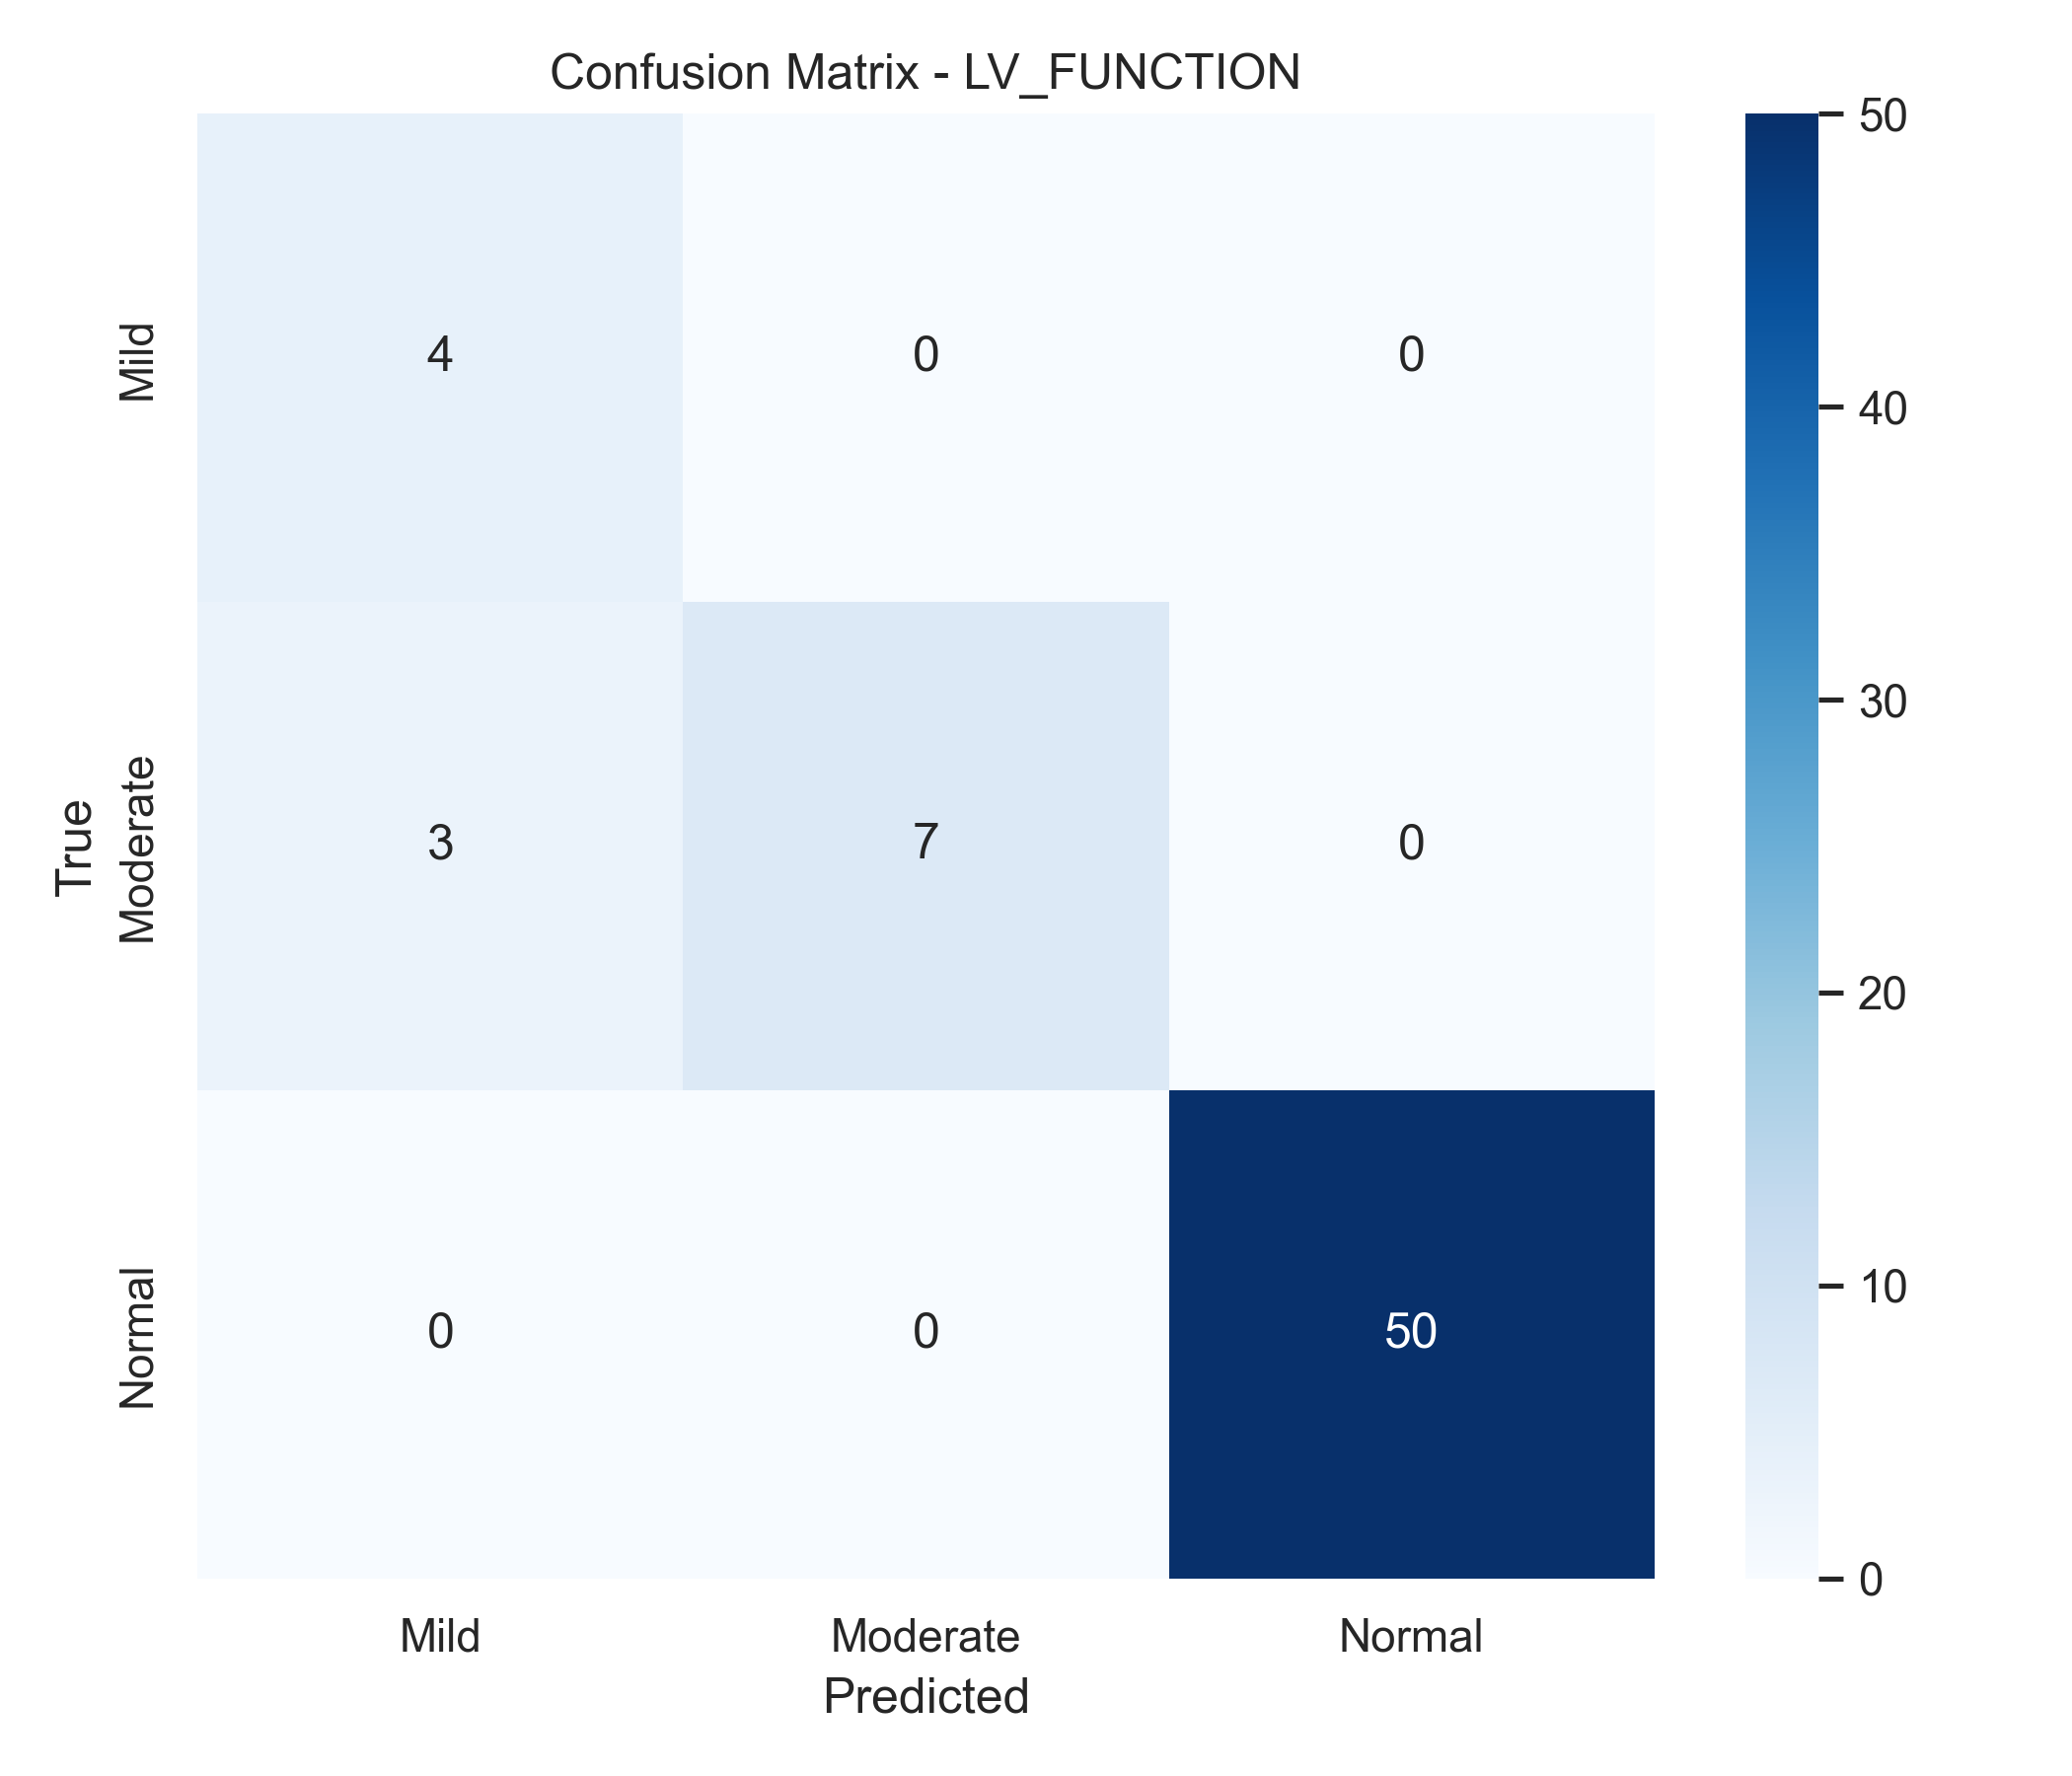
\includegraphics[width=\textwidth]{../../outputs/paper_plots/confusion_matrix_LV_FUNCTION.png}
\caption{LV\_FUNCTION}
\end{subfigure}
\begin{subfigure}[b]{0.19\textwidth}
\includegraphics[width=\textwidth]{../../outputs/paper_plots/confusion_matrix_LV_SIZE.png}
\caption{LV\_SIZE}
\end{subfigure}
\begin{subfigure}[b]{0.19\textwidth}
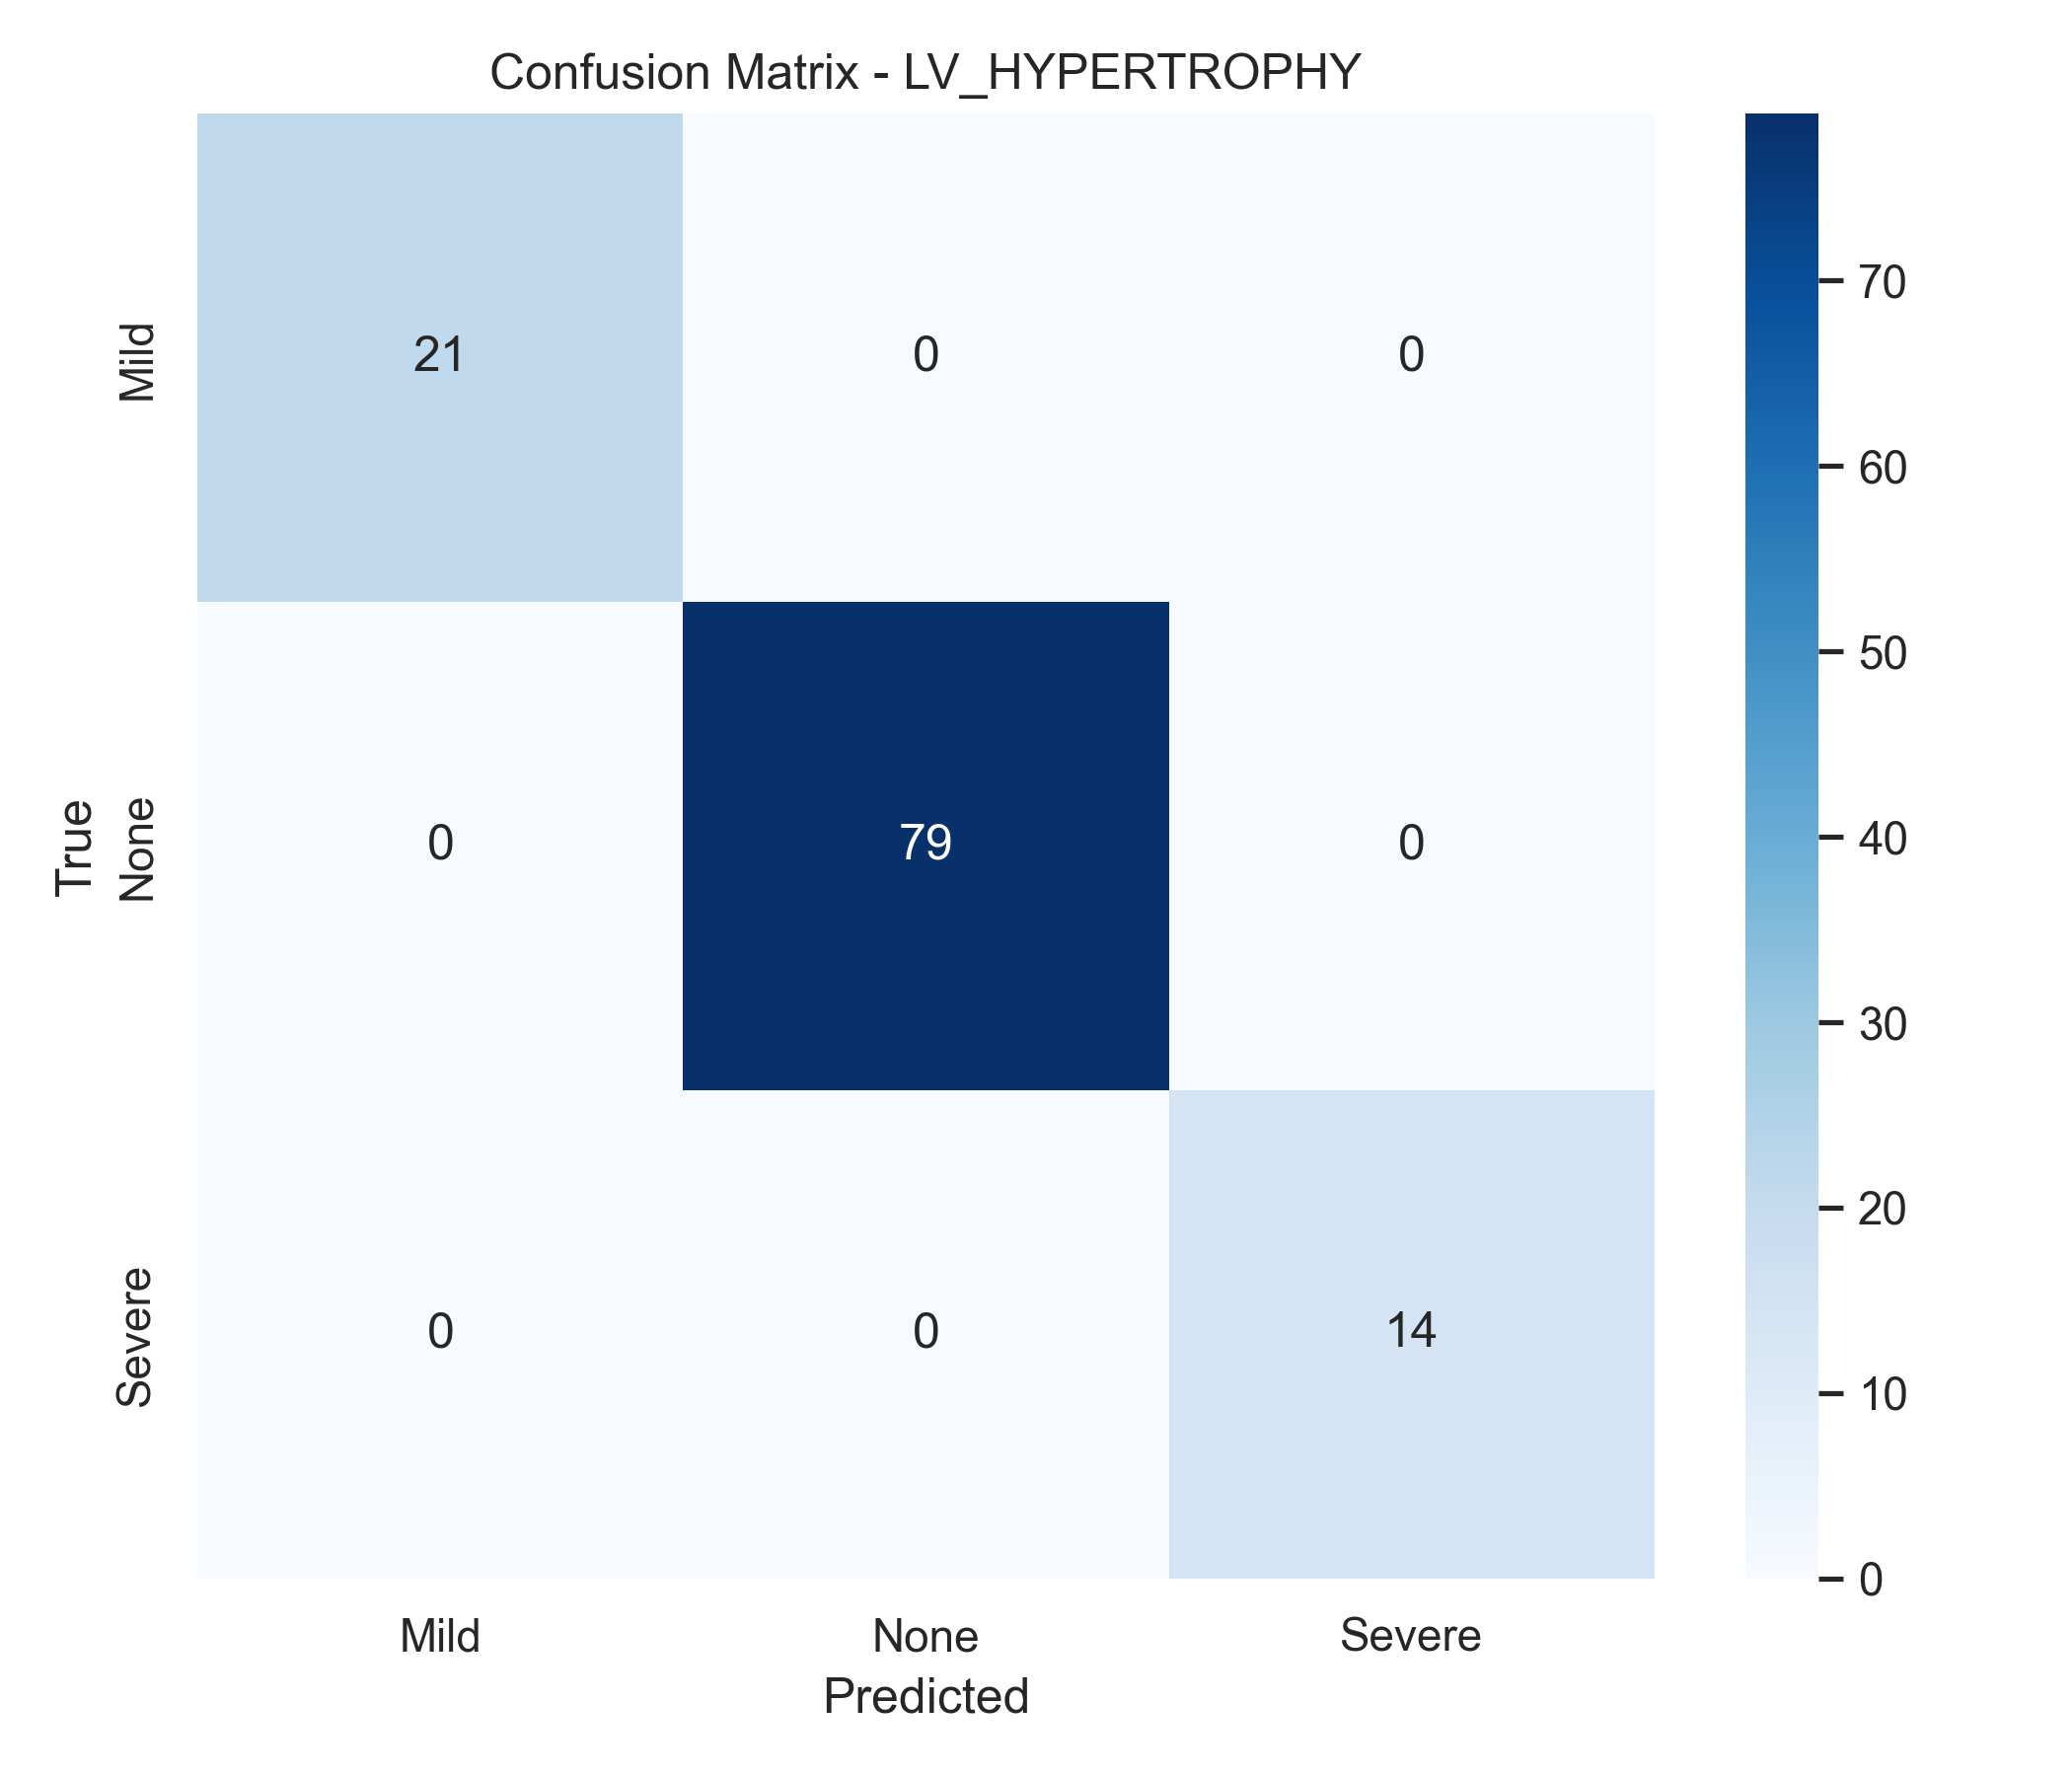
\includegraphics[width=\textwidth]{../../outputs/paper_plots/confusion_matrix_LV_HYPERTROPHY.png}
\caption{LV\_HYPERTROPHY}
\end{subfigure}
\begin{subfigure}[b]{0.19\textwidth}
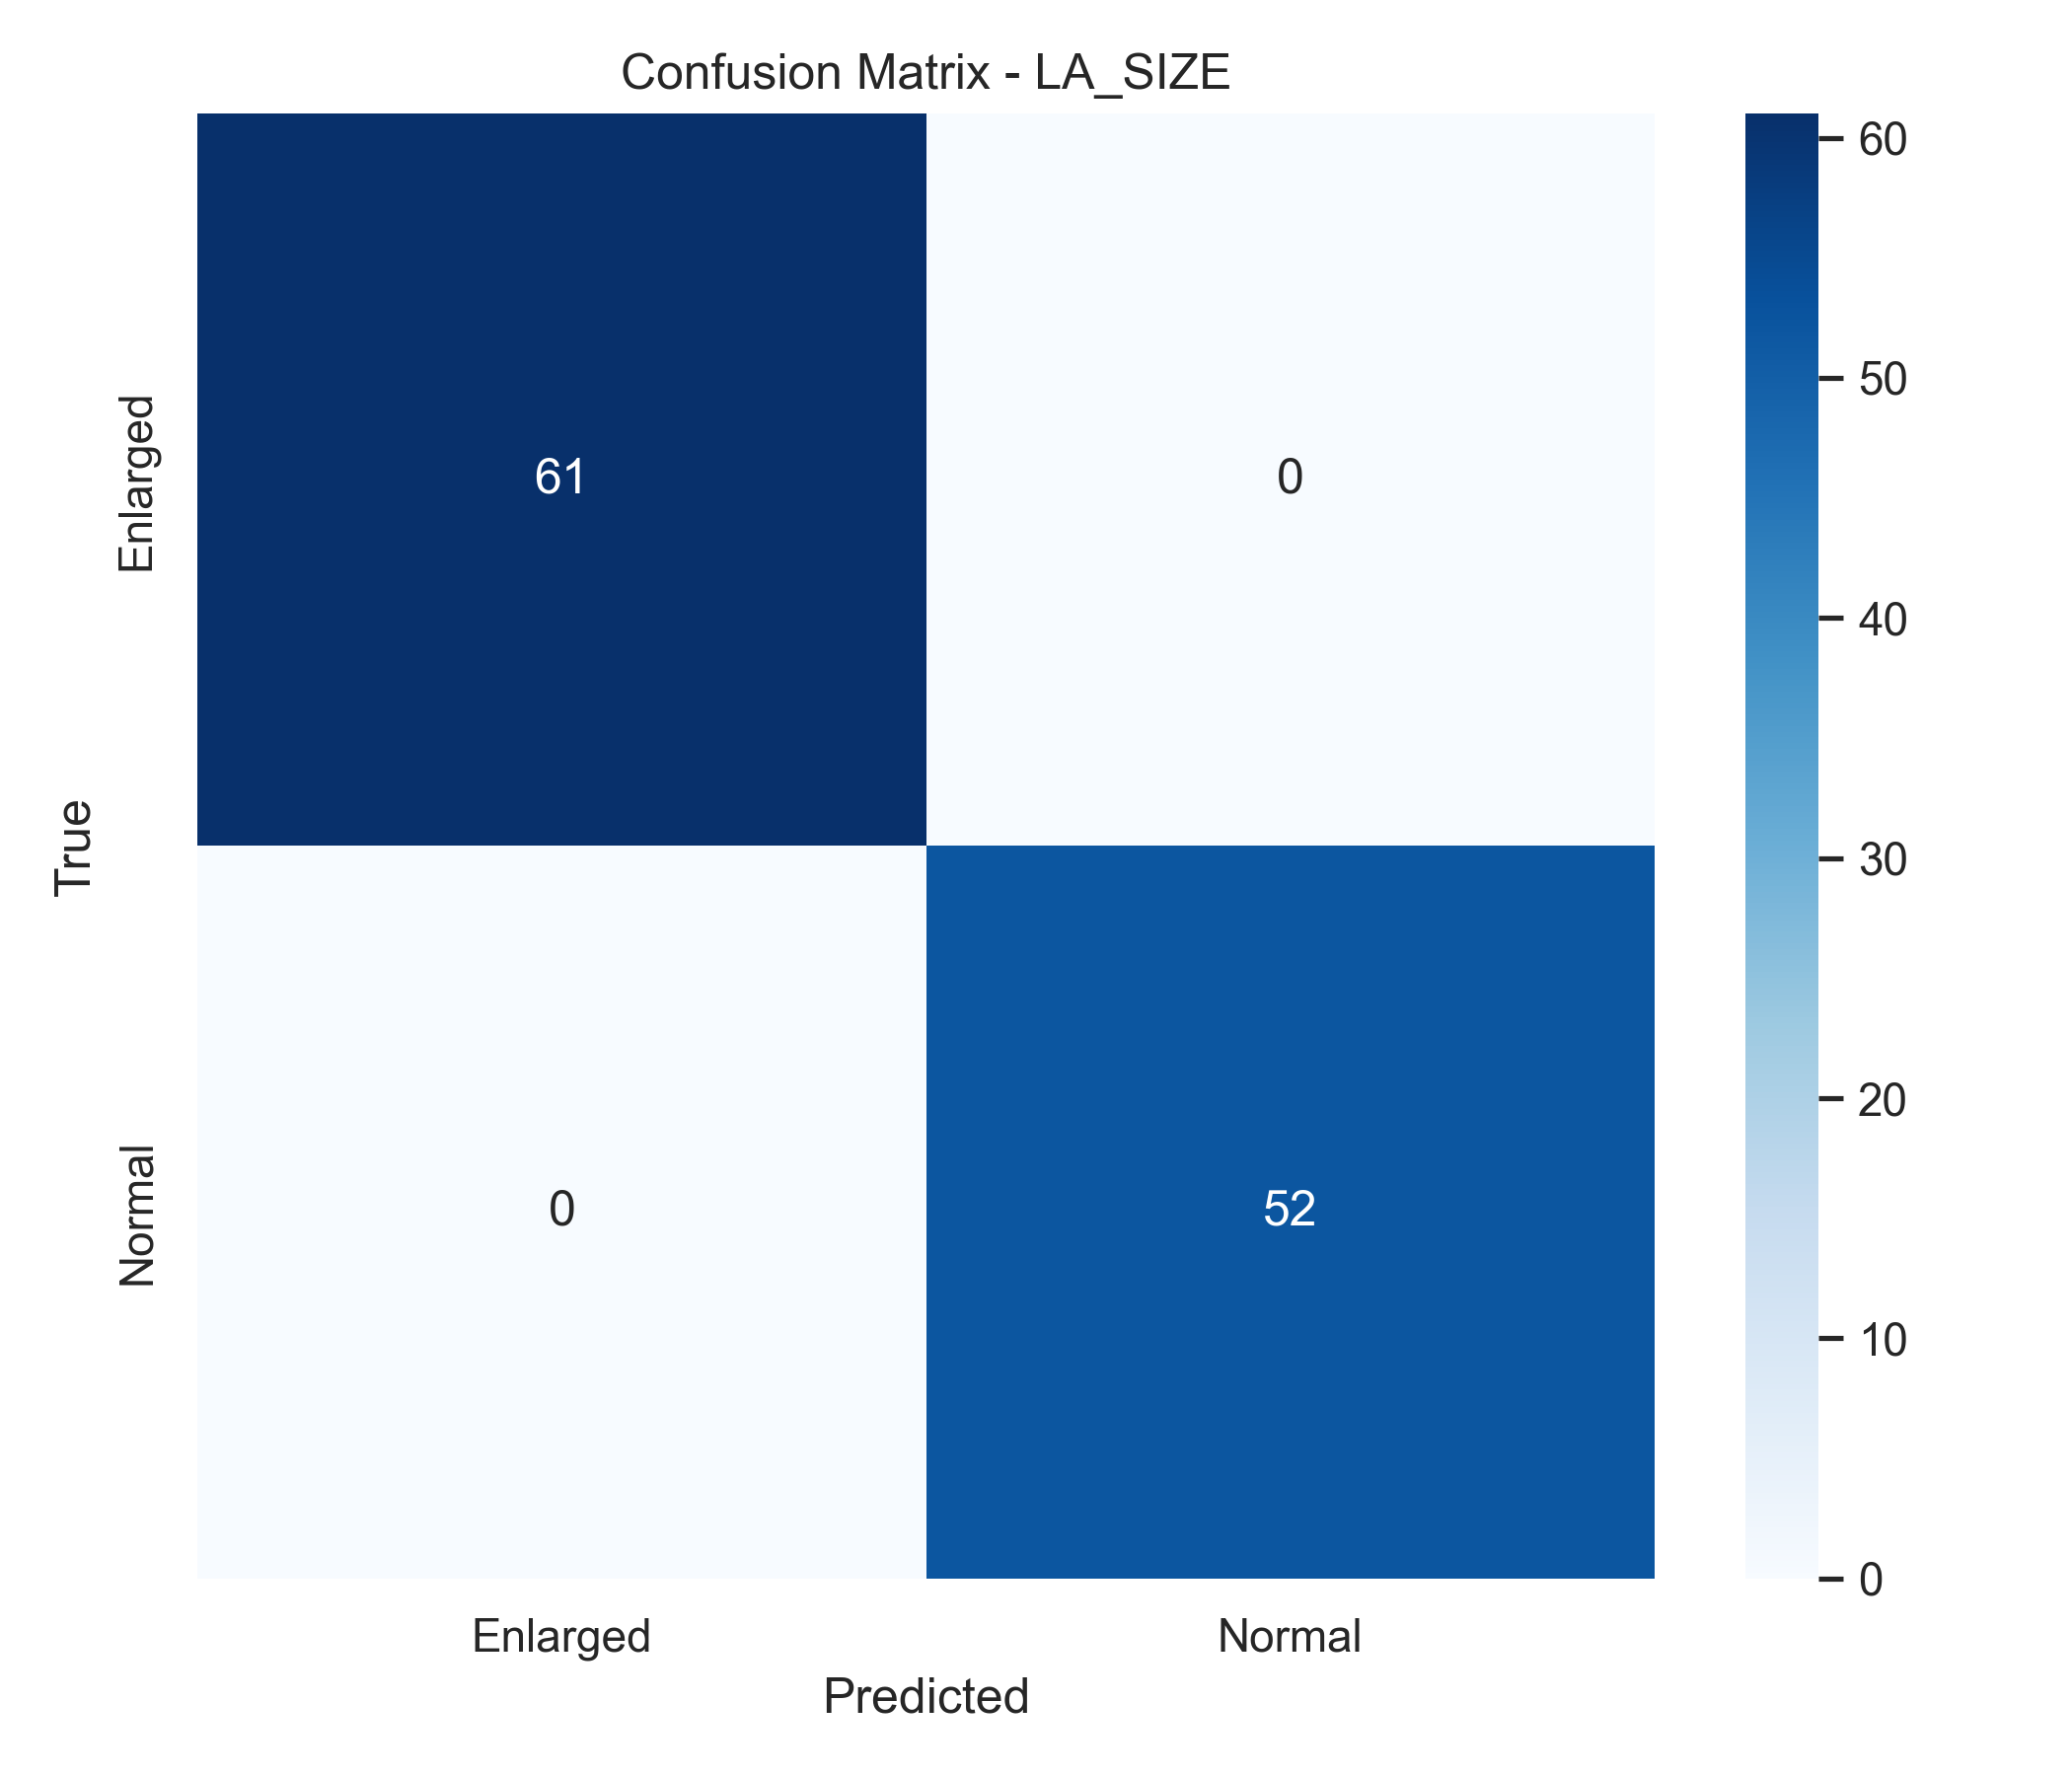
\includegraphics[width=\textwidth]{../../outputs/paper_plots/confusion_matrix_LA_SIZE.png}
\caption{LA\_SIZE}
\end{subfigure}
\begin{subfigure}[b]{0.19\textwidth}
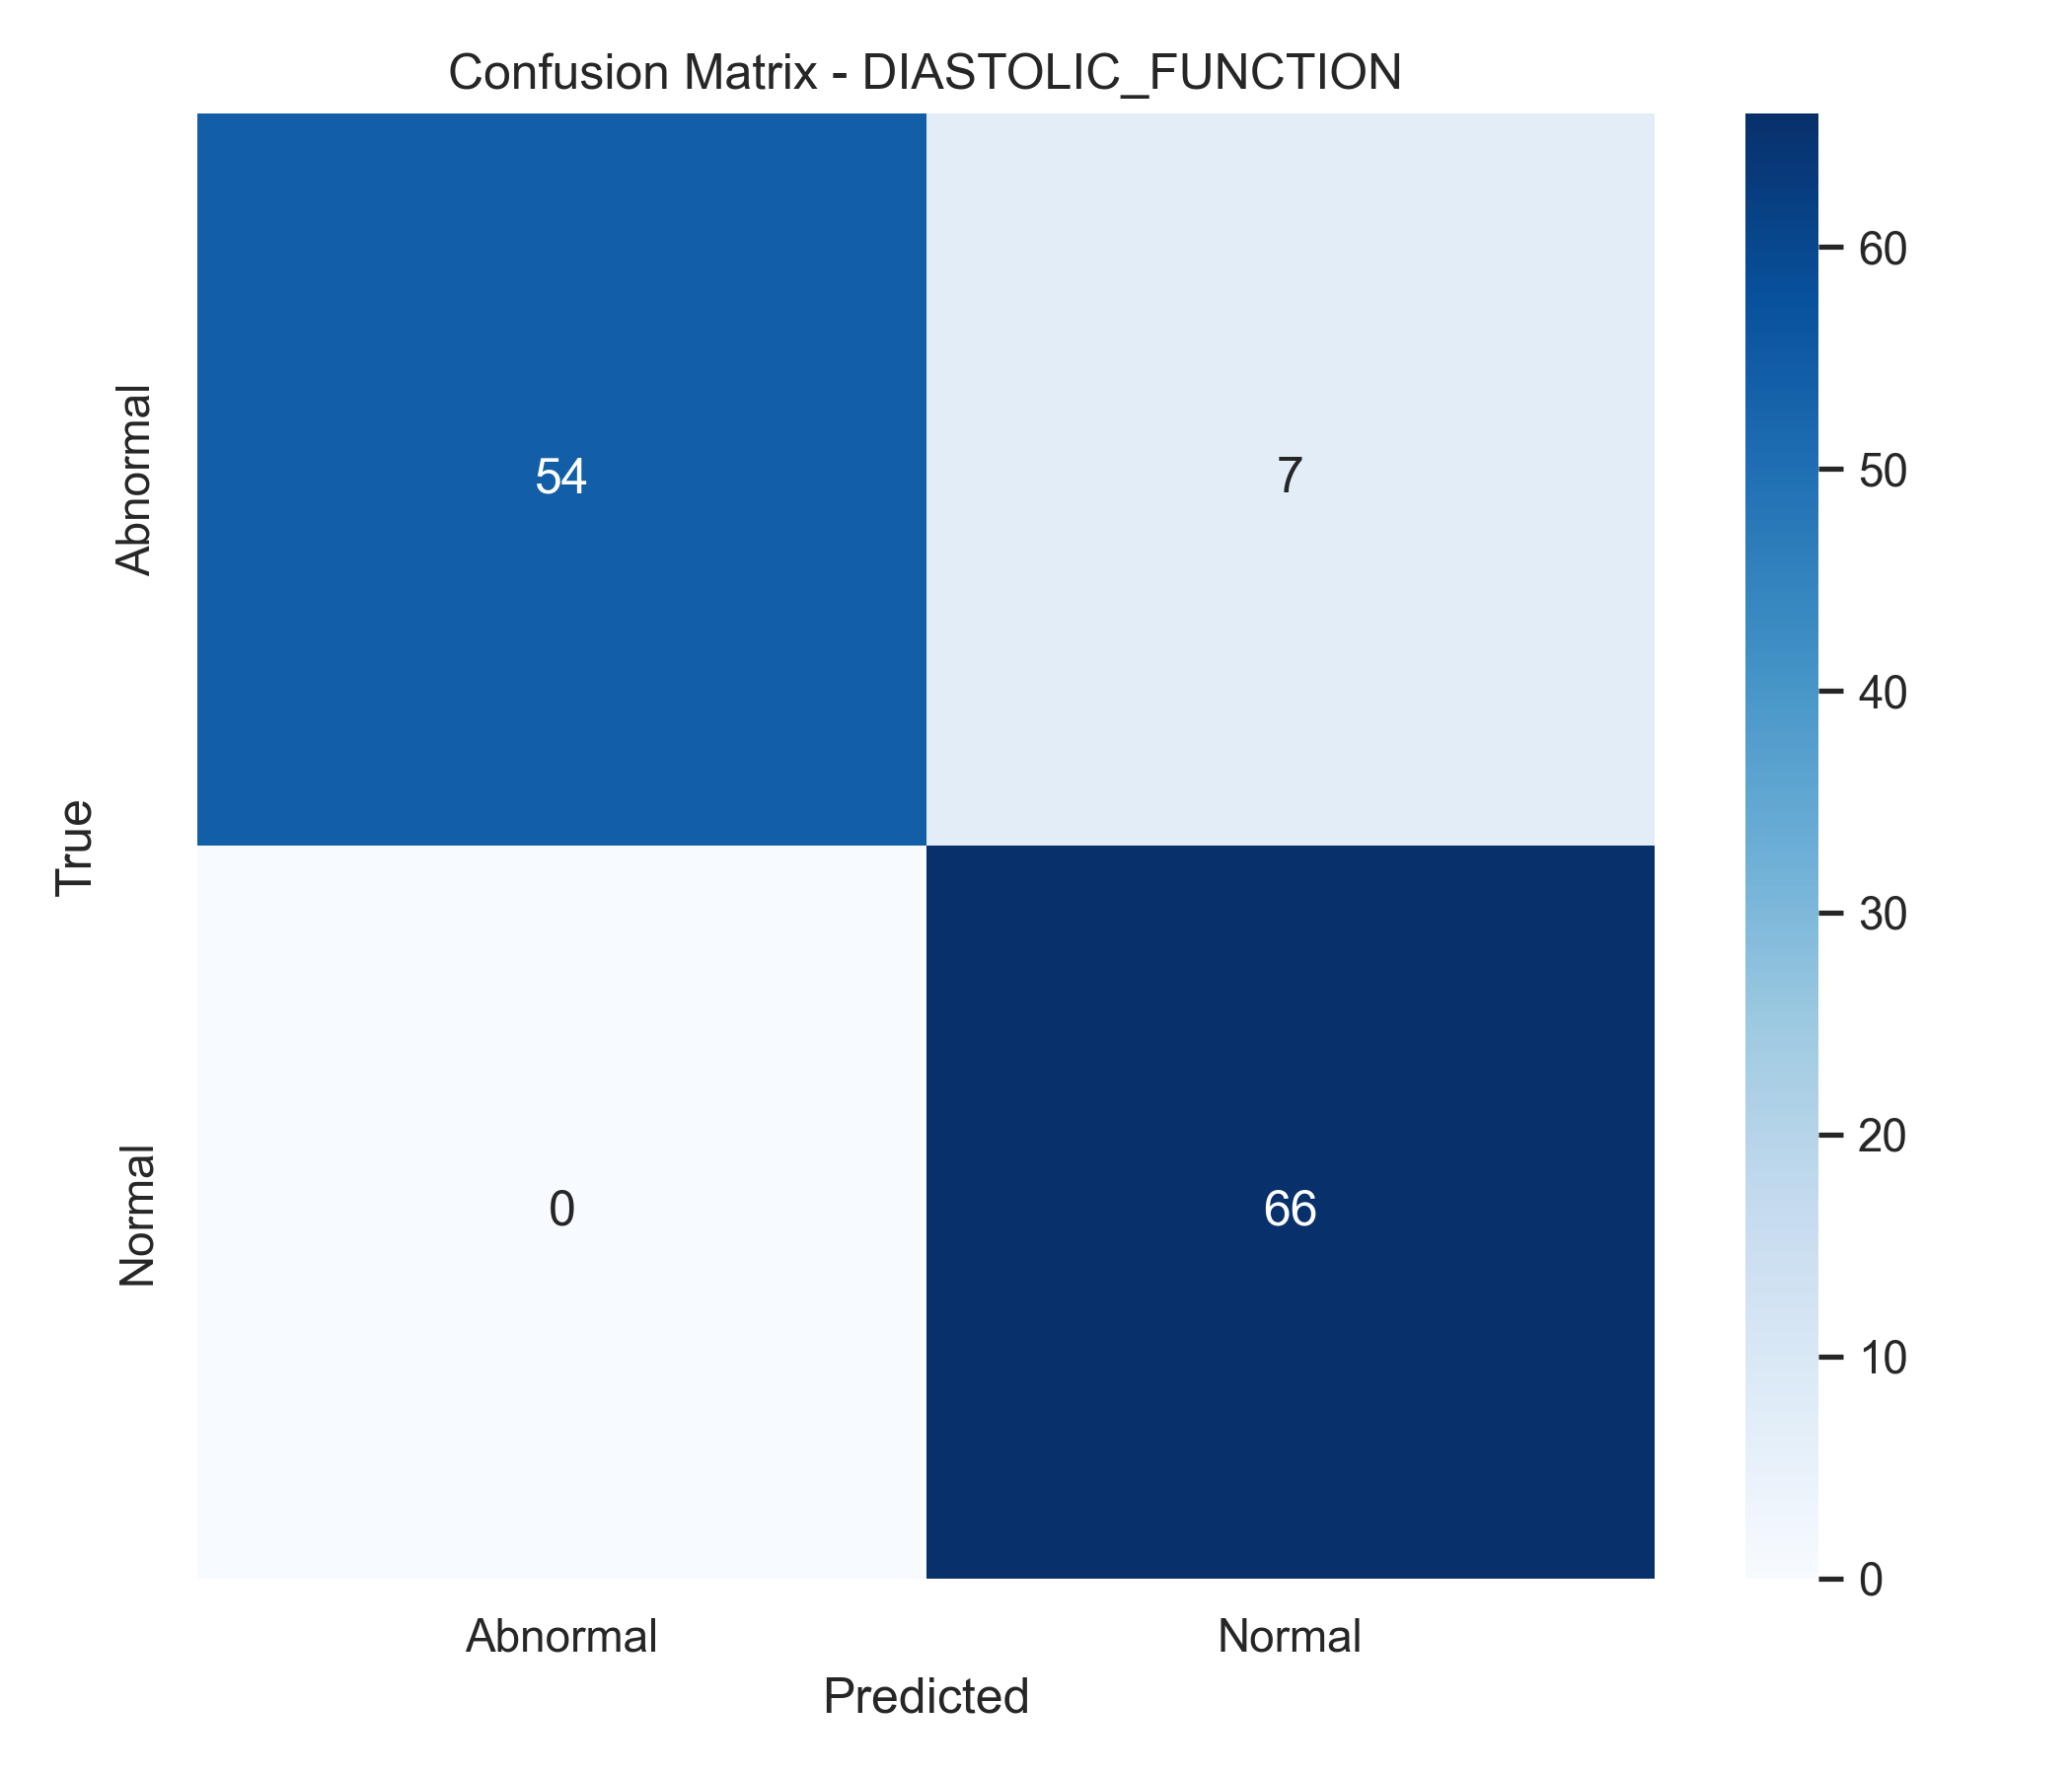
\includegraphics[width=\textwidth]{../../outputs/paper_plots/confusion_matrix_DIASTOLIC_FUNCTION.png}
\caption{DIASTOLIC\_FN}
\end{subfigure}
\caption{Confusion matrices for all five prediction categories (expanded benchmark).}
\label{fig:confusion}
\end{figure*}

\begin{figure*}[t]
\centering
\begin{subfigure}[b]{0.19\textwidth}
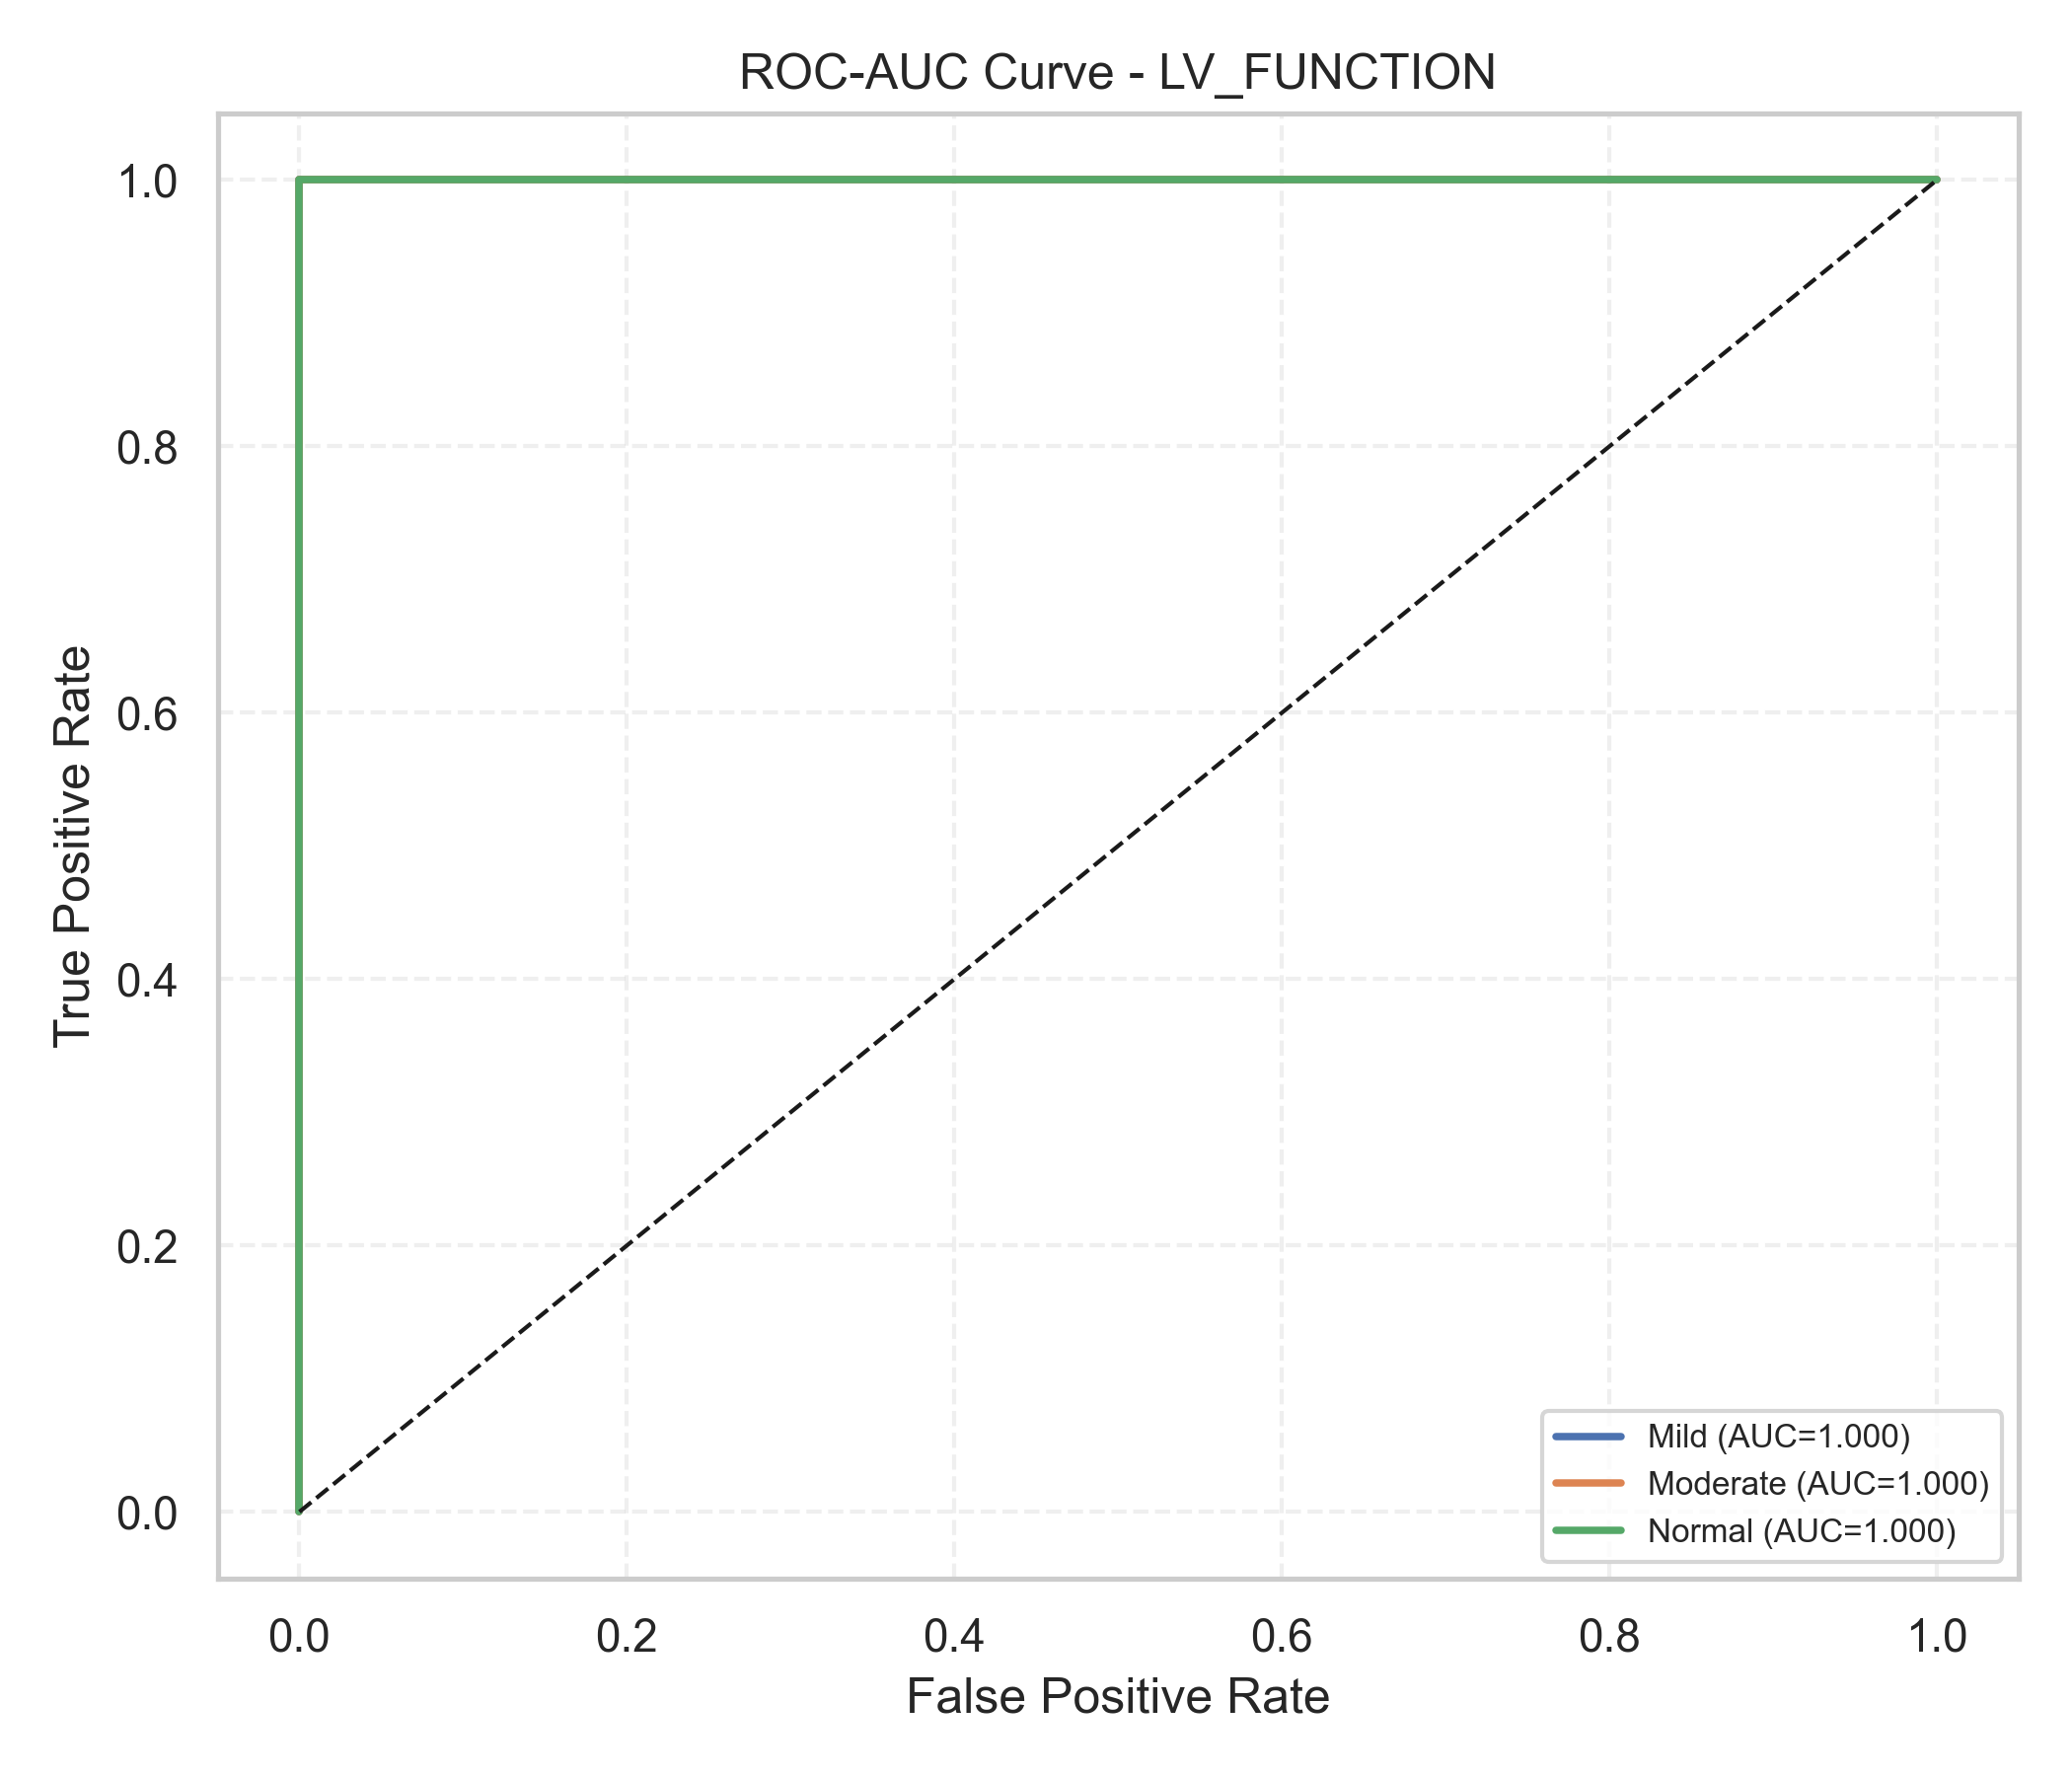
\includegraphics[width=\textwidth]{../../outputs/paper_plots/roc_auc_LV_FUNCTION.png}
\caption{LV\_FUNCTION}
\end{subfigure}
\begin{subfigure}[b]{0.19\textwidth}
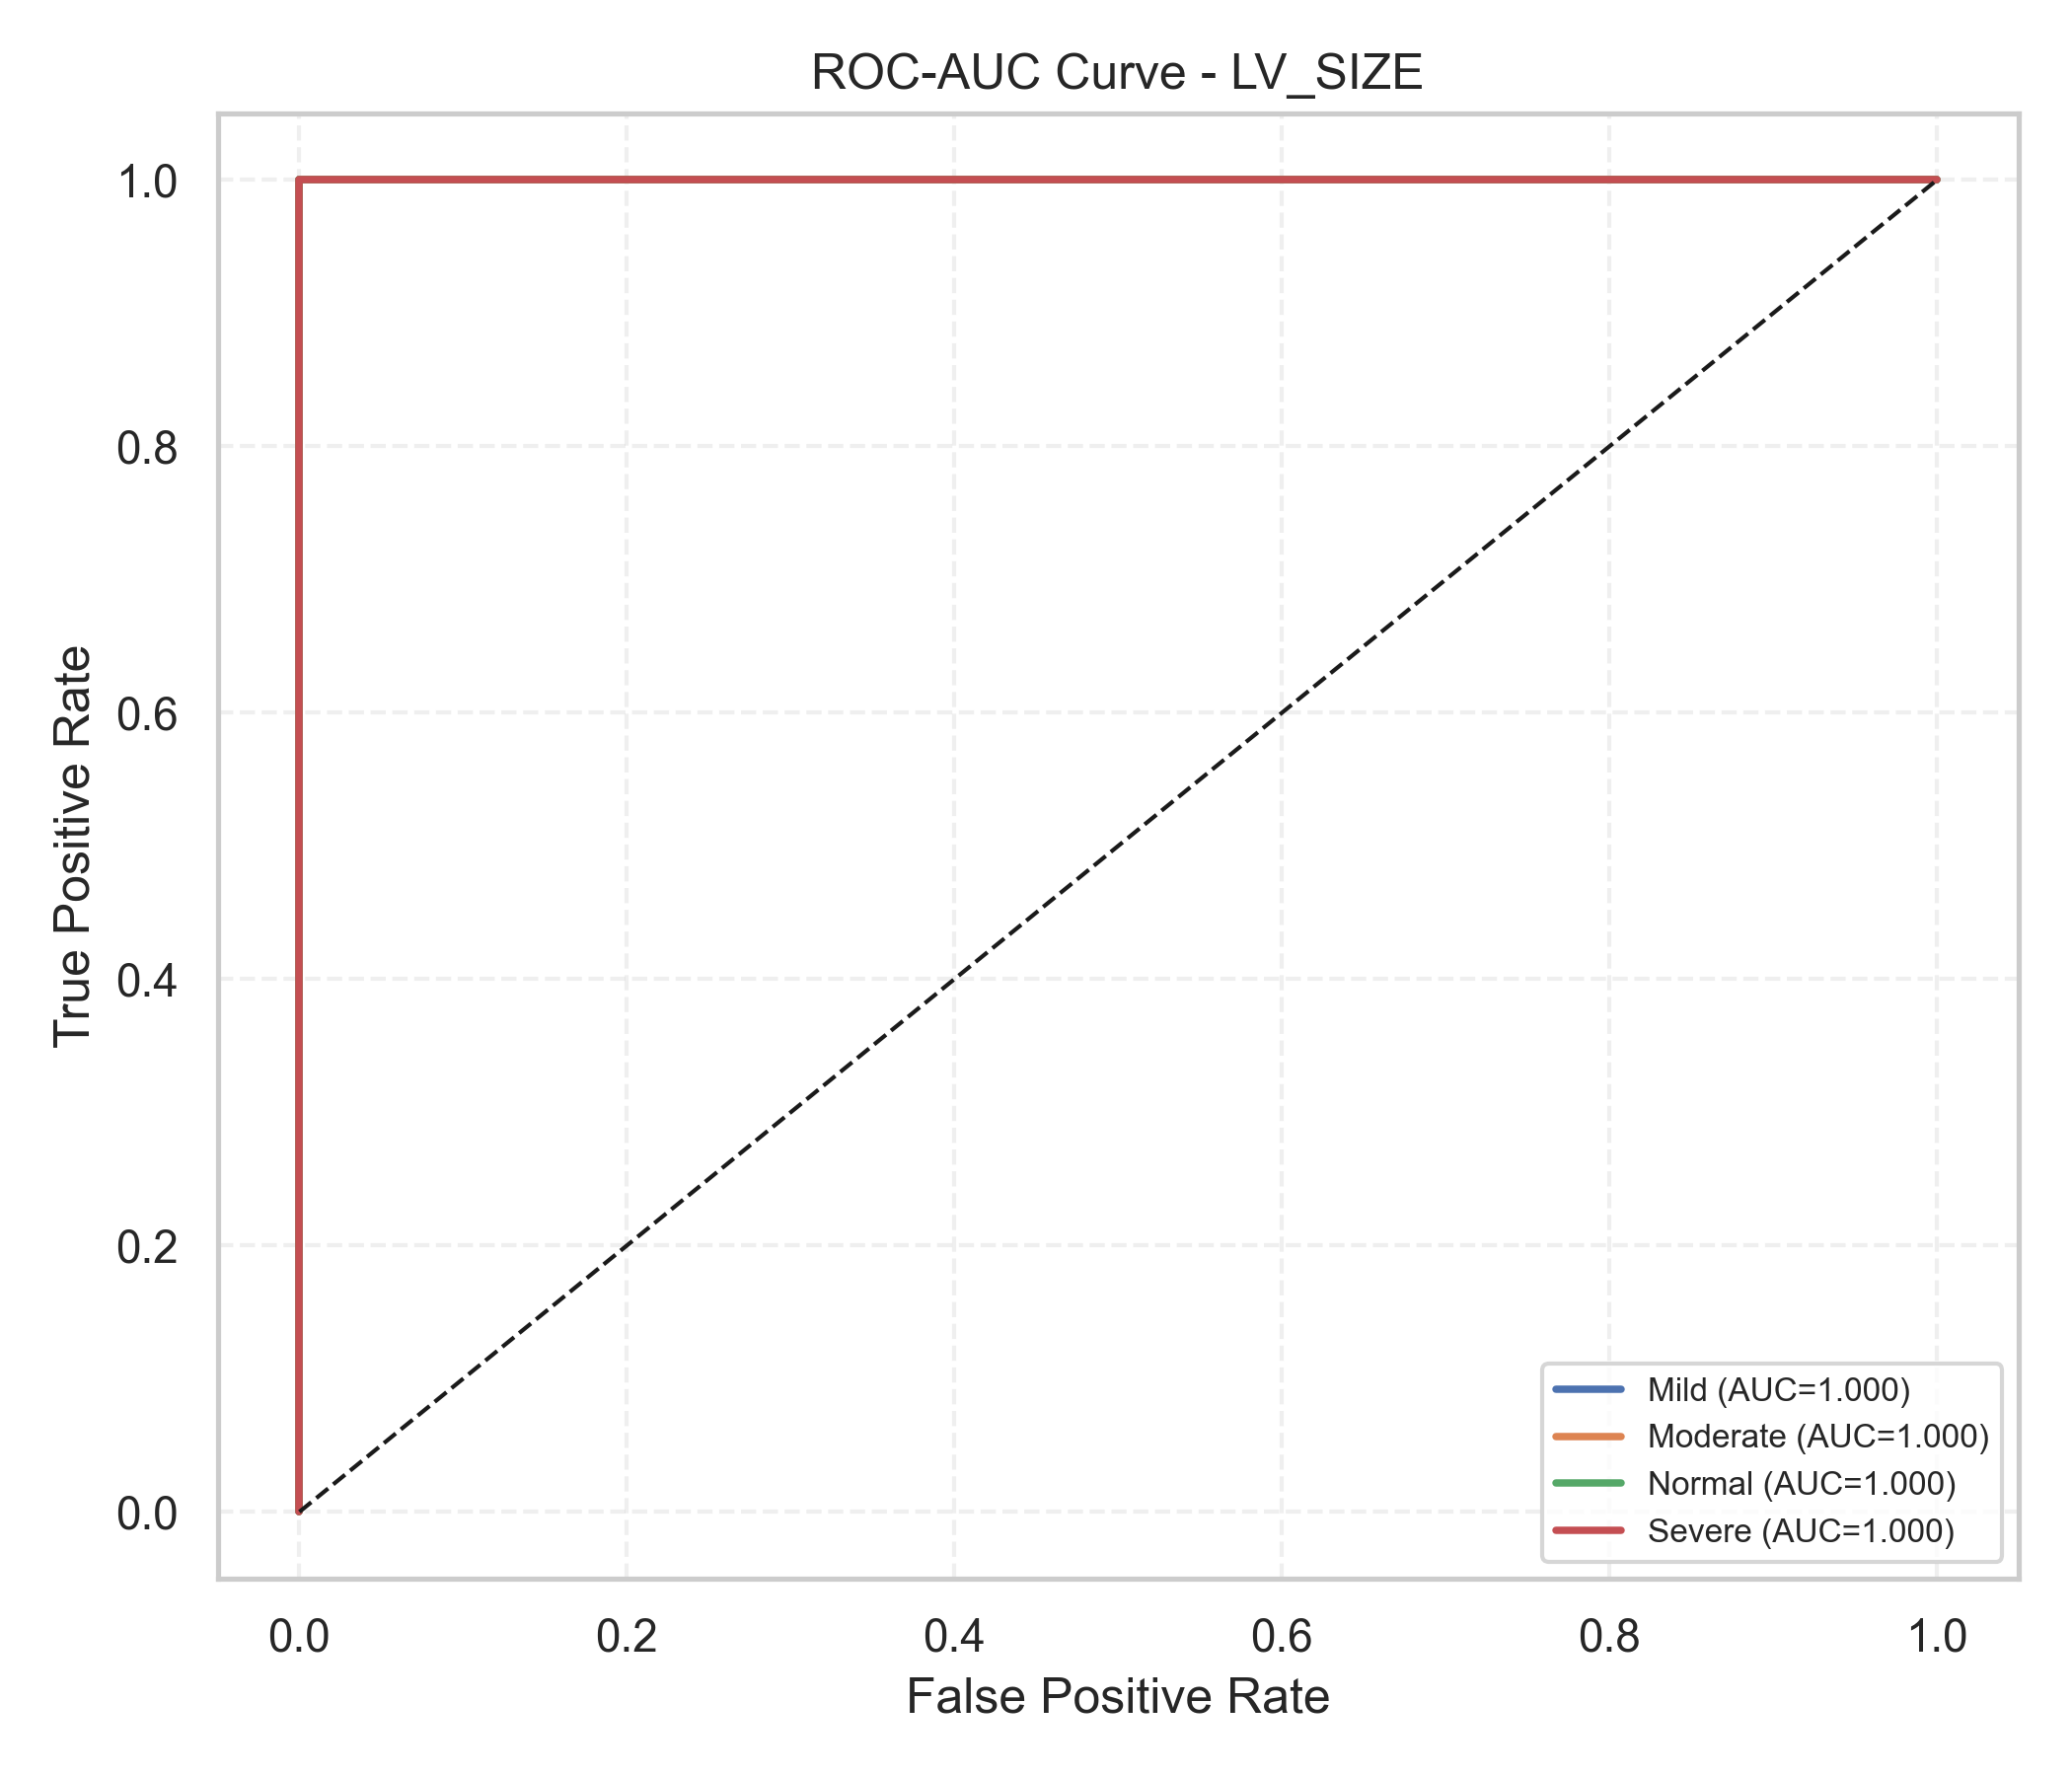
\includegraphics[width=\textwidth]{../../outputs/paper_plots/roc_auc_LV_SIZE.png}
\caption{LV\_SIZE}
\end{subfigure}
\begin{subfigure}[b]{0.19\textwidth}
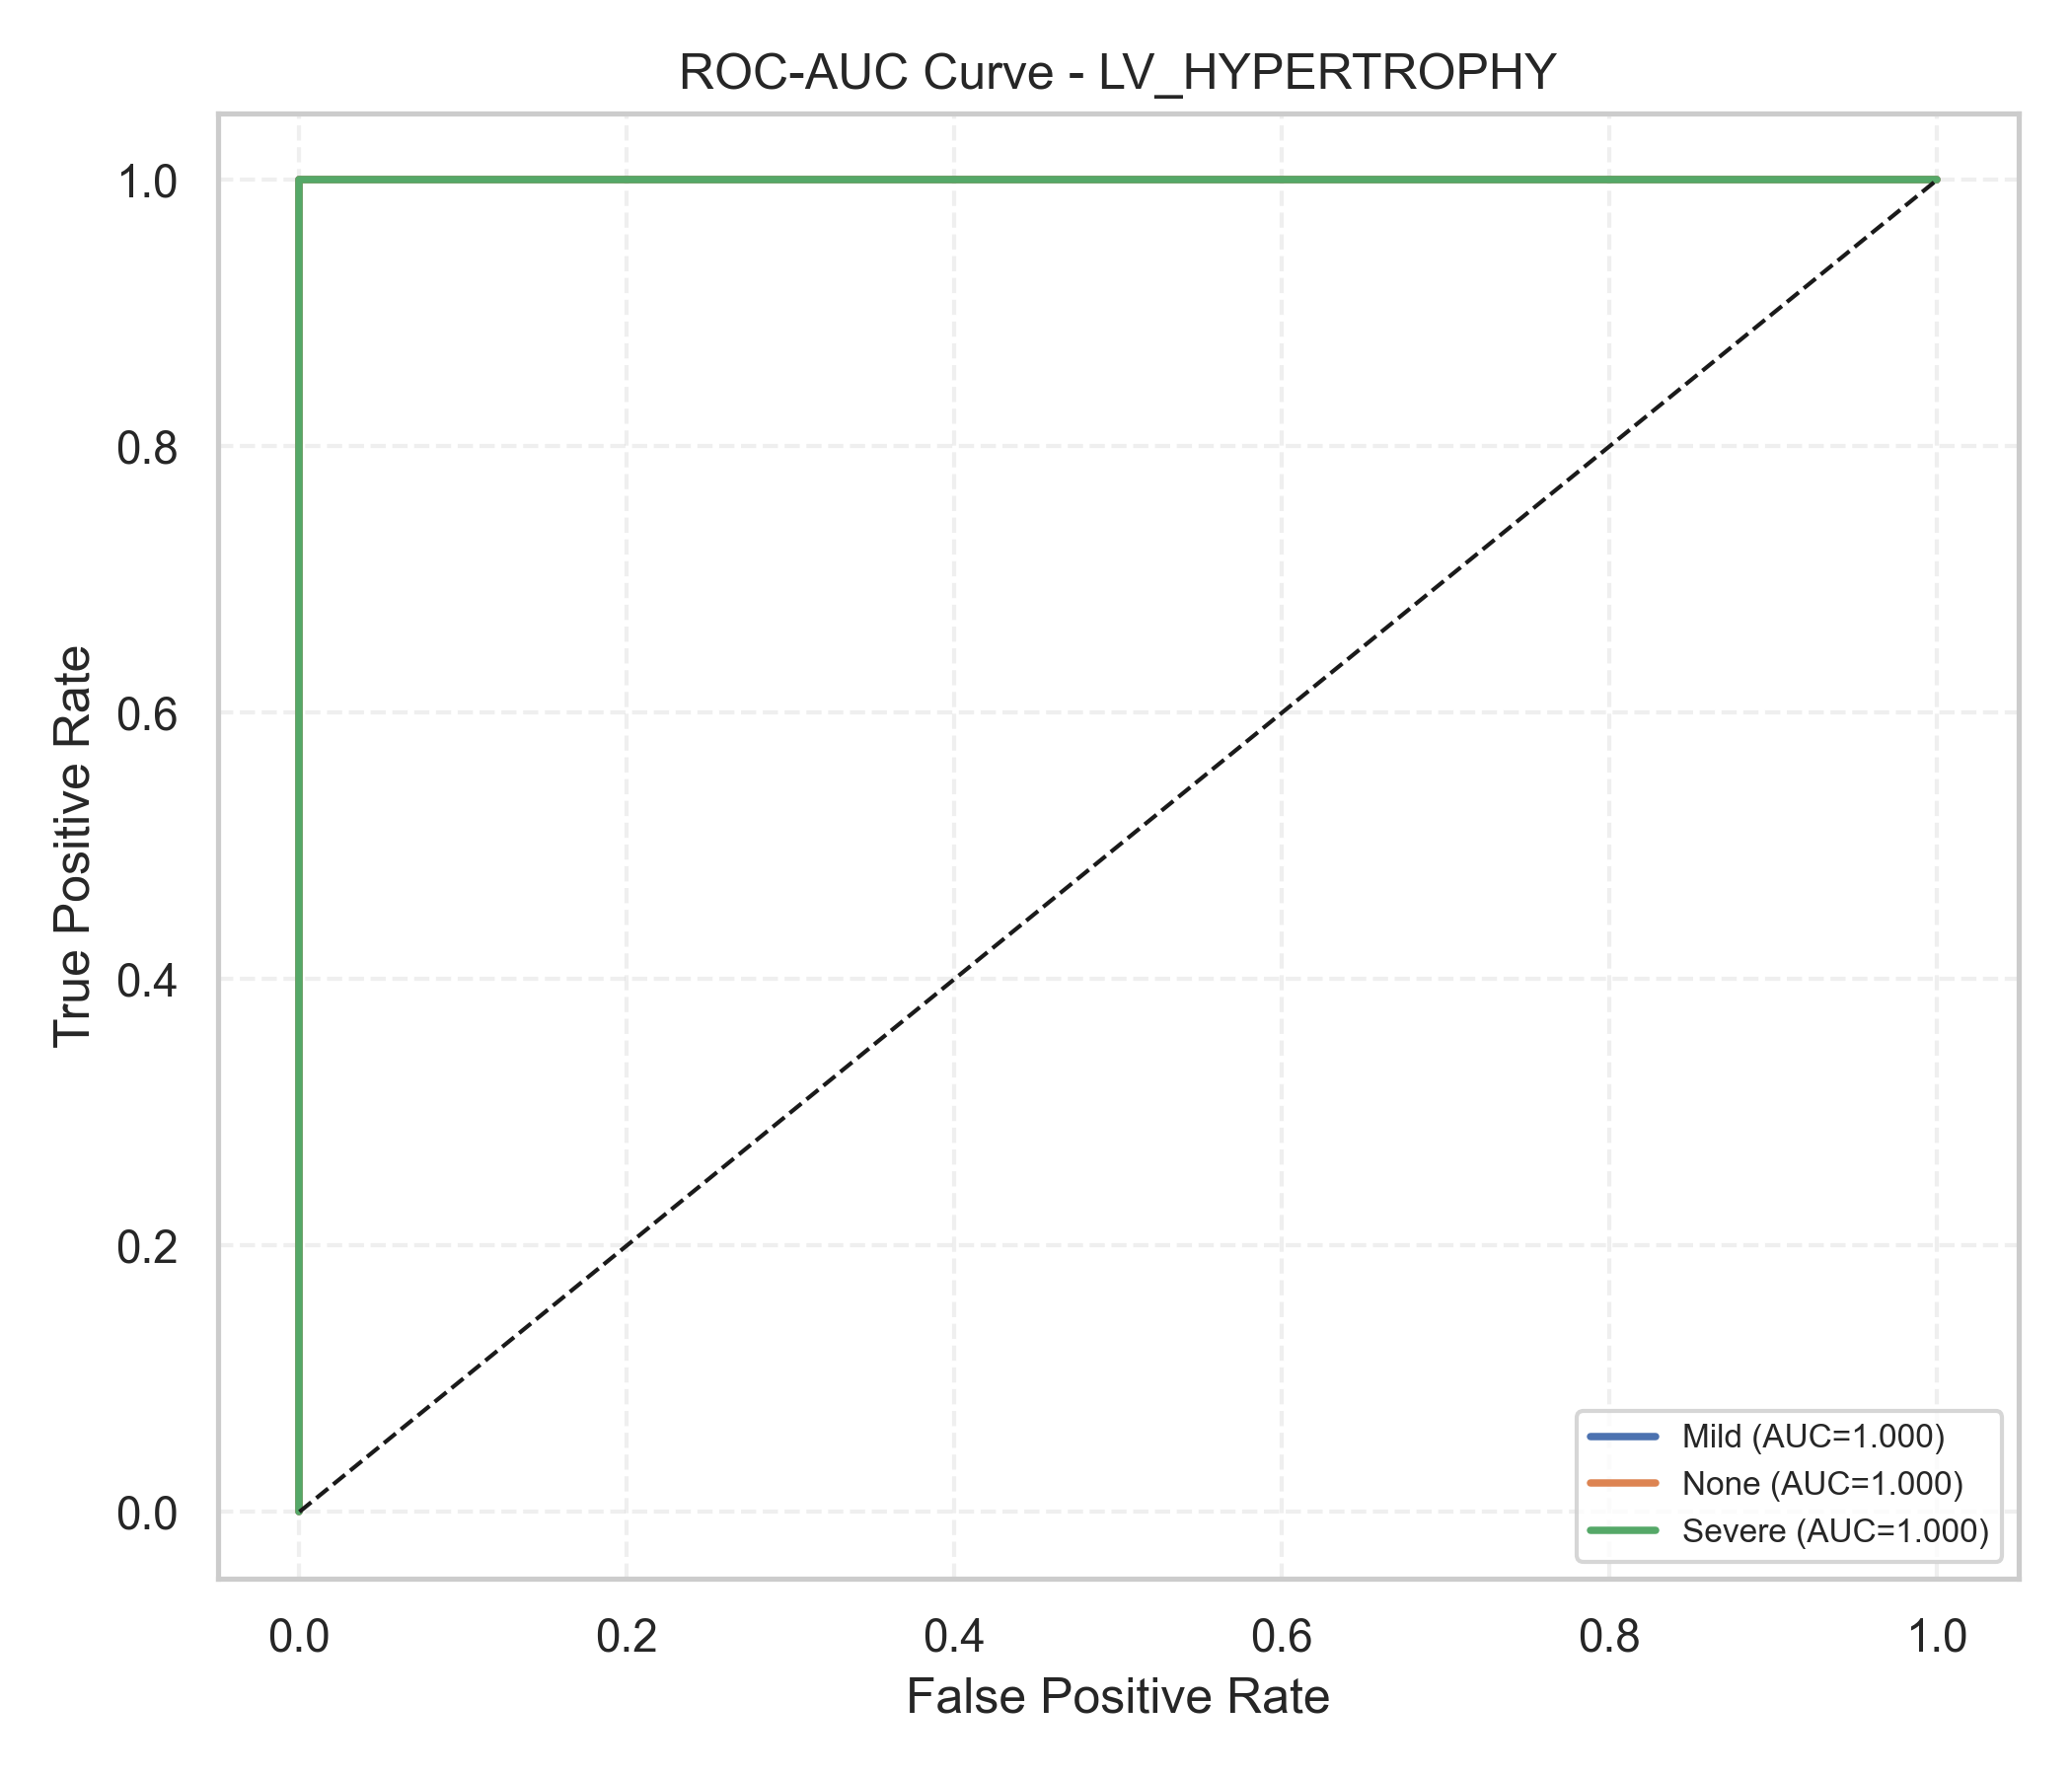
\includegraphics[width=\textwidth]{../../outputs/paper_plots/roc_auc_LV_HYPERTROPHY.png}
\caption{LV\_HYPERTROPHY}
\end{subfigure}
\begin{subfigure}[b]{0.19\textwidth}
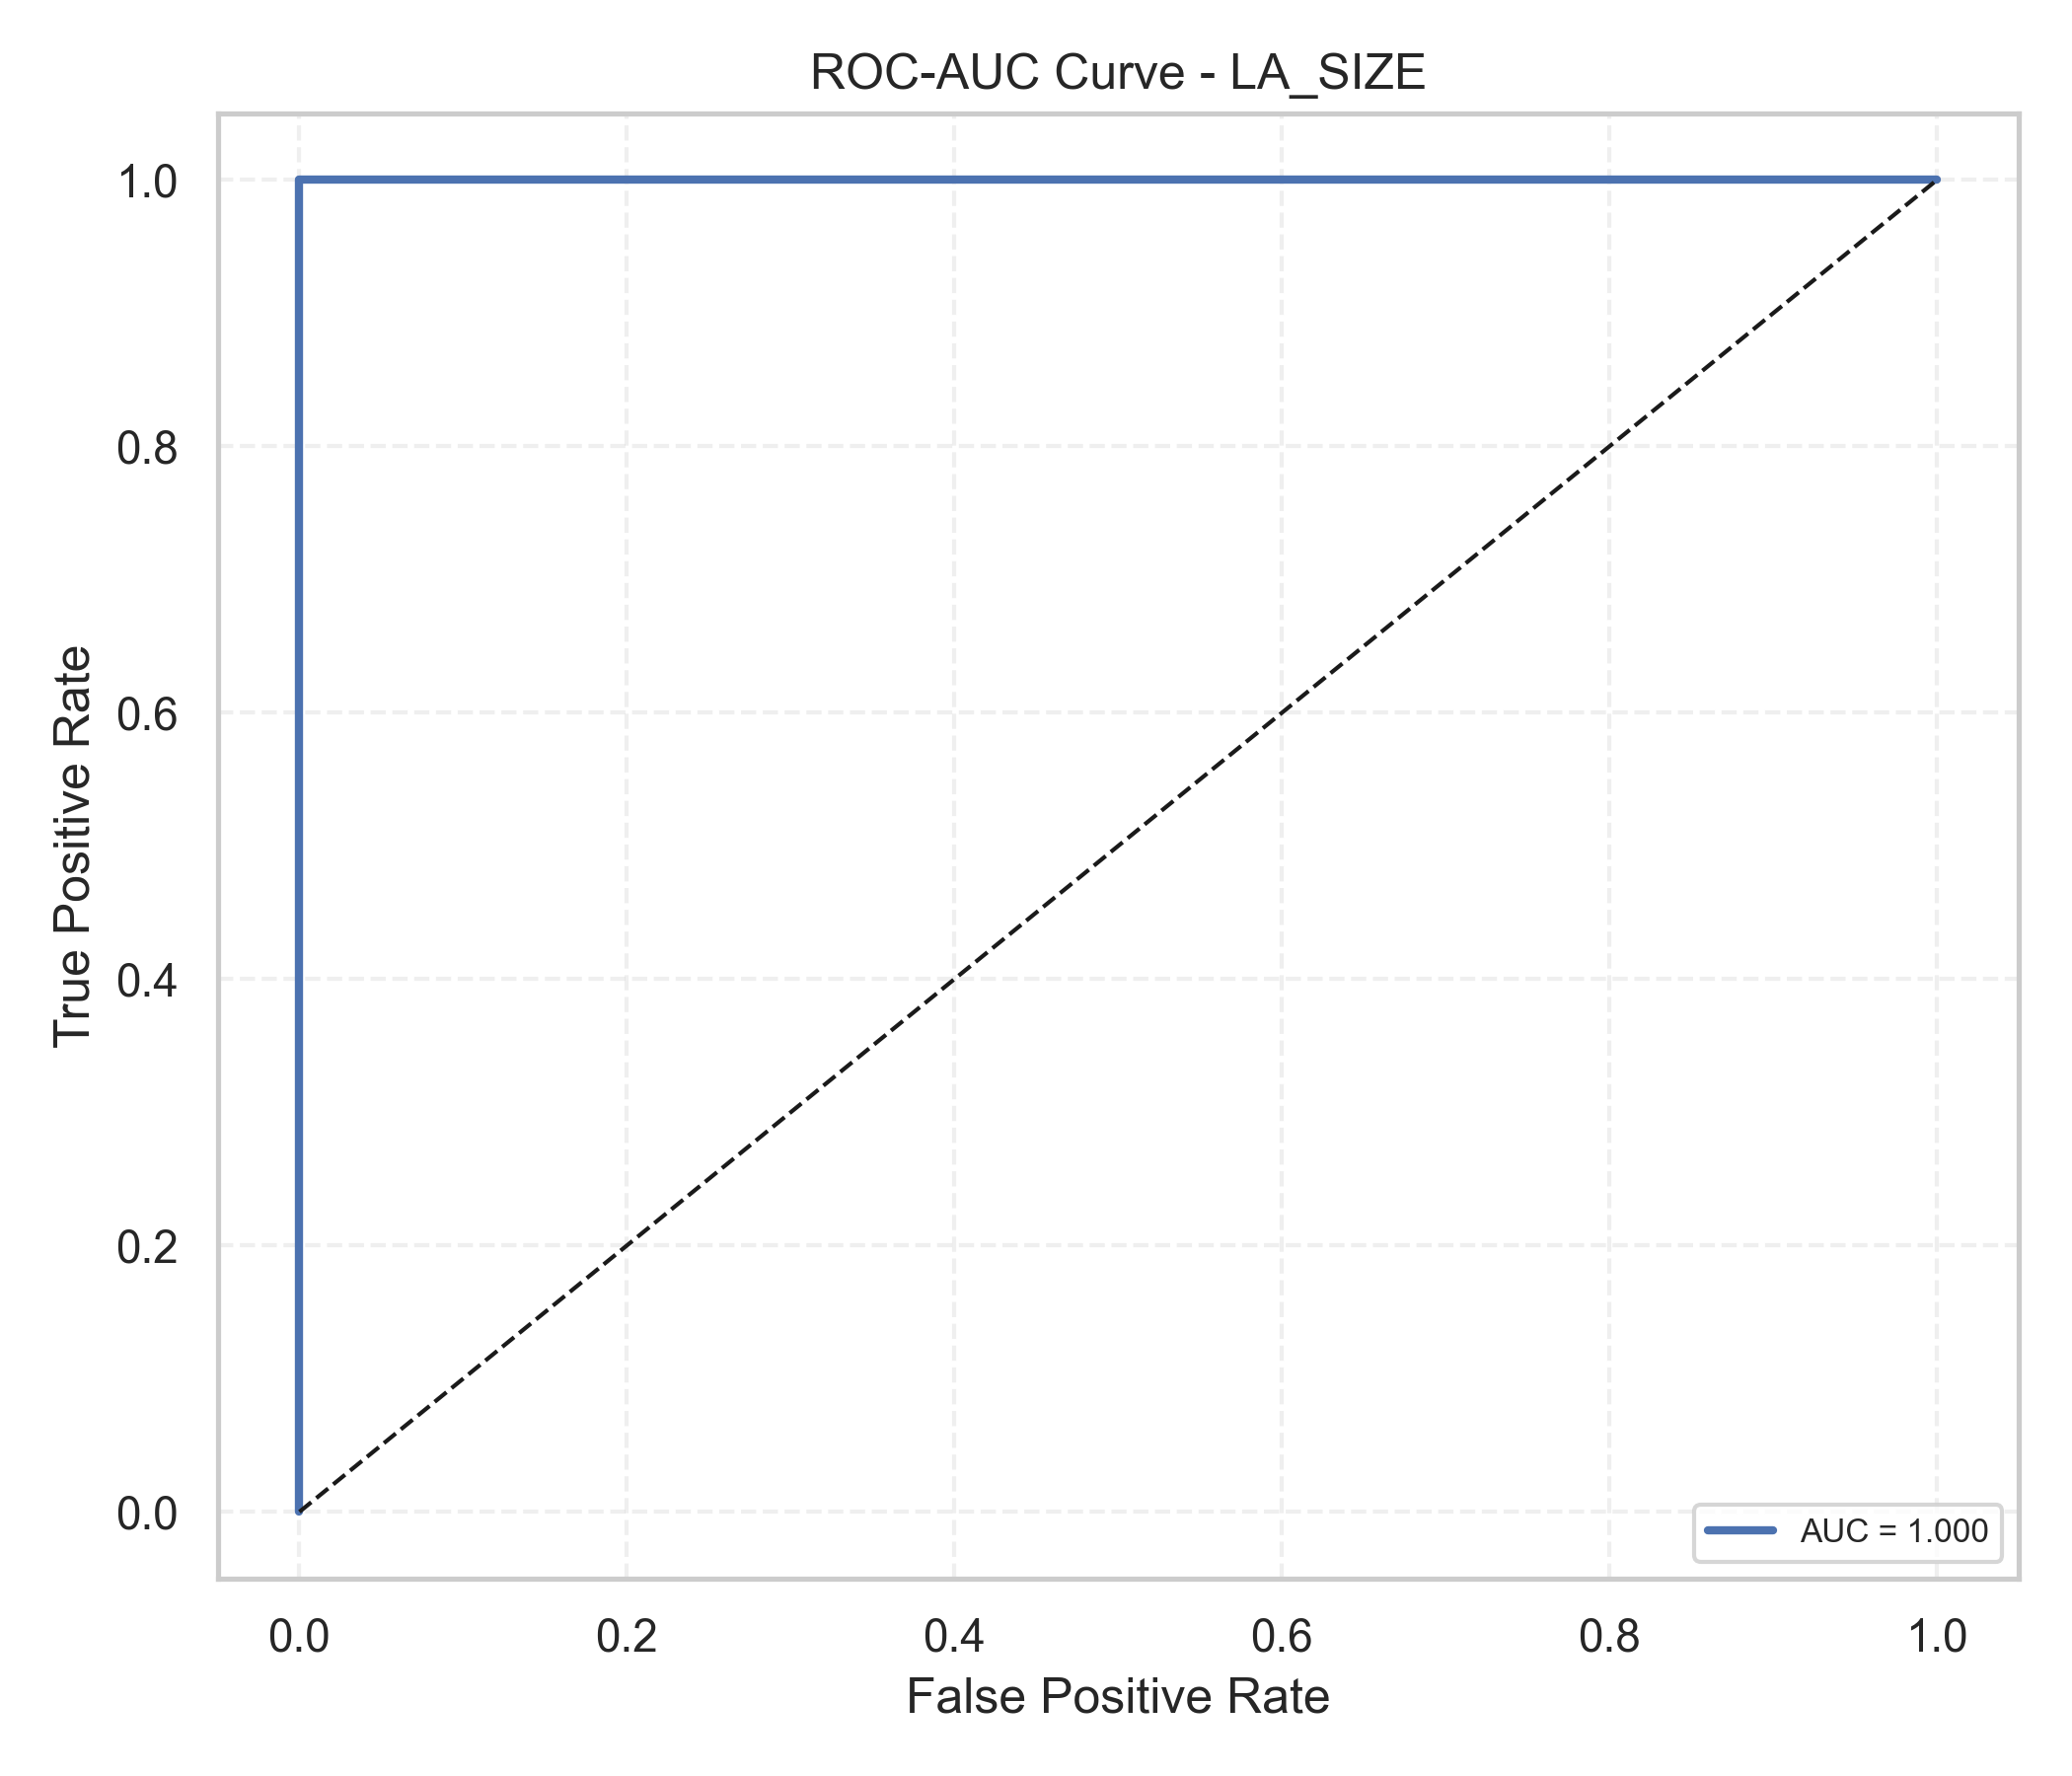
\includegraphics[width=\textwidth]{../../outputs/paper_plots/roc_auc_LA_SIZE.png}
\caption{LA\_SIZE}
\end{subfigure}
\begin{subfigure}[b]{0.19\textwidth}
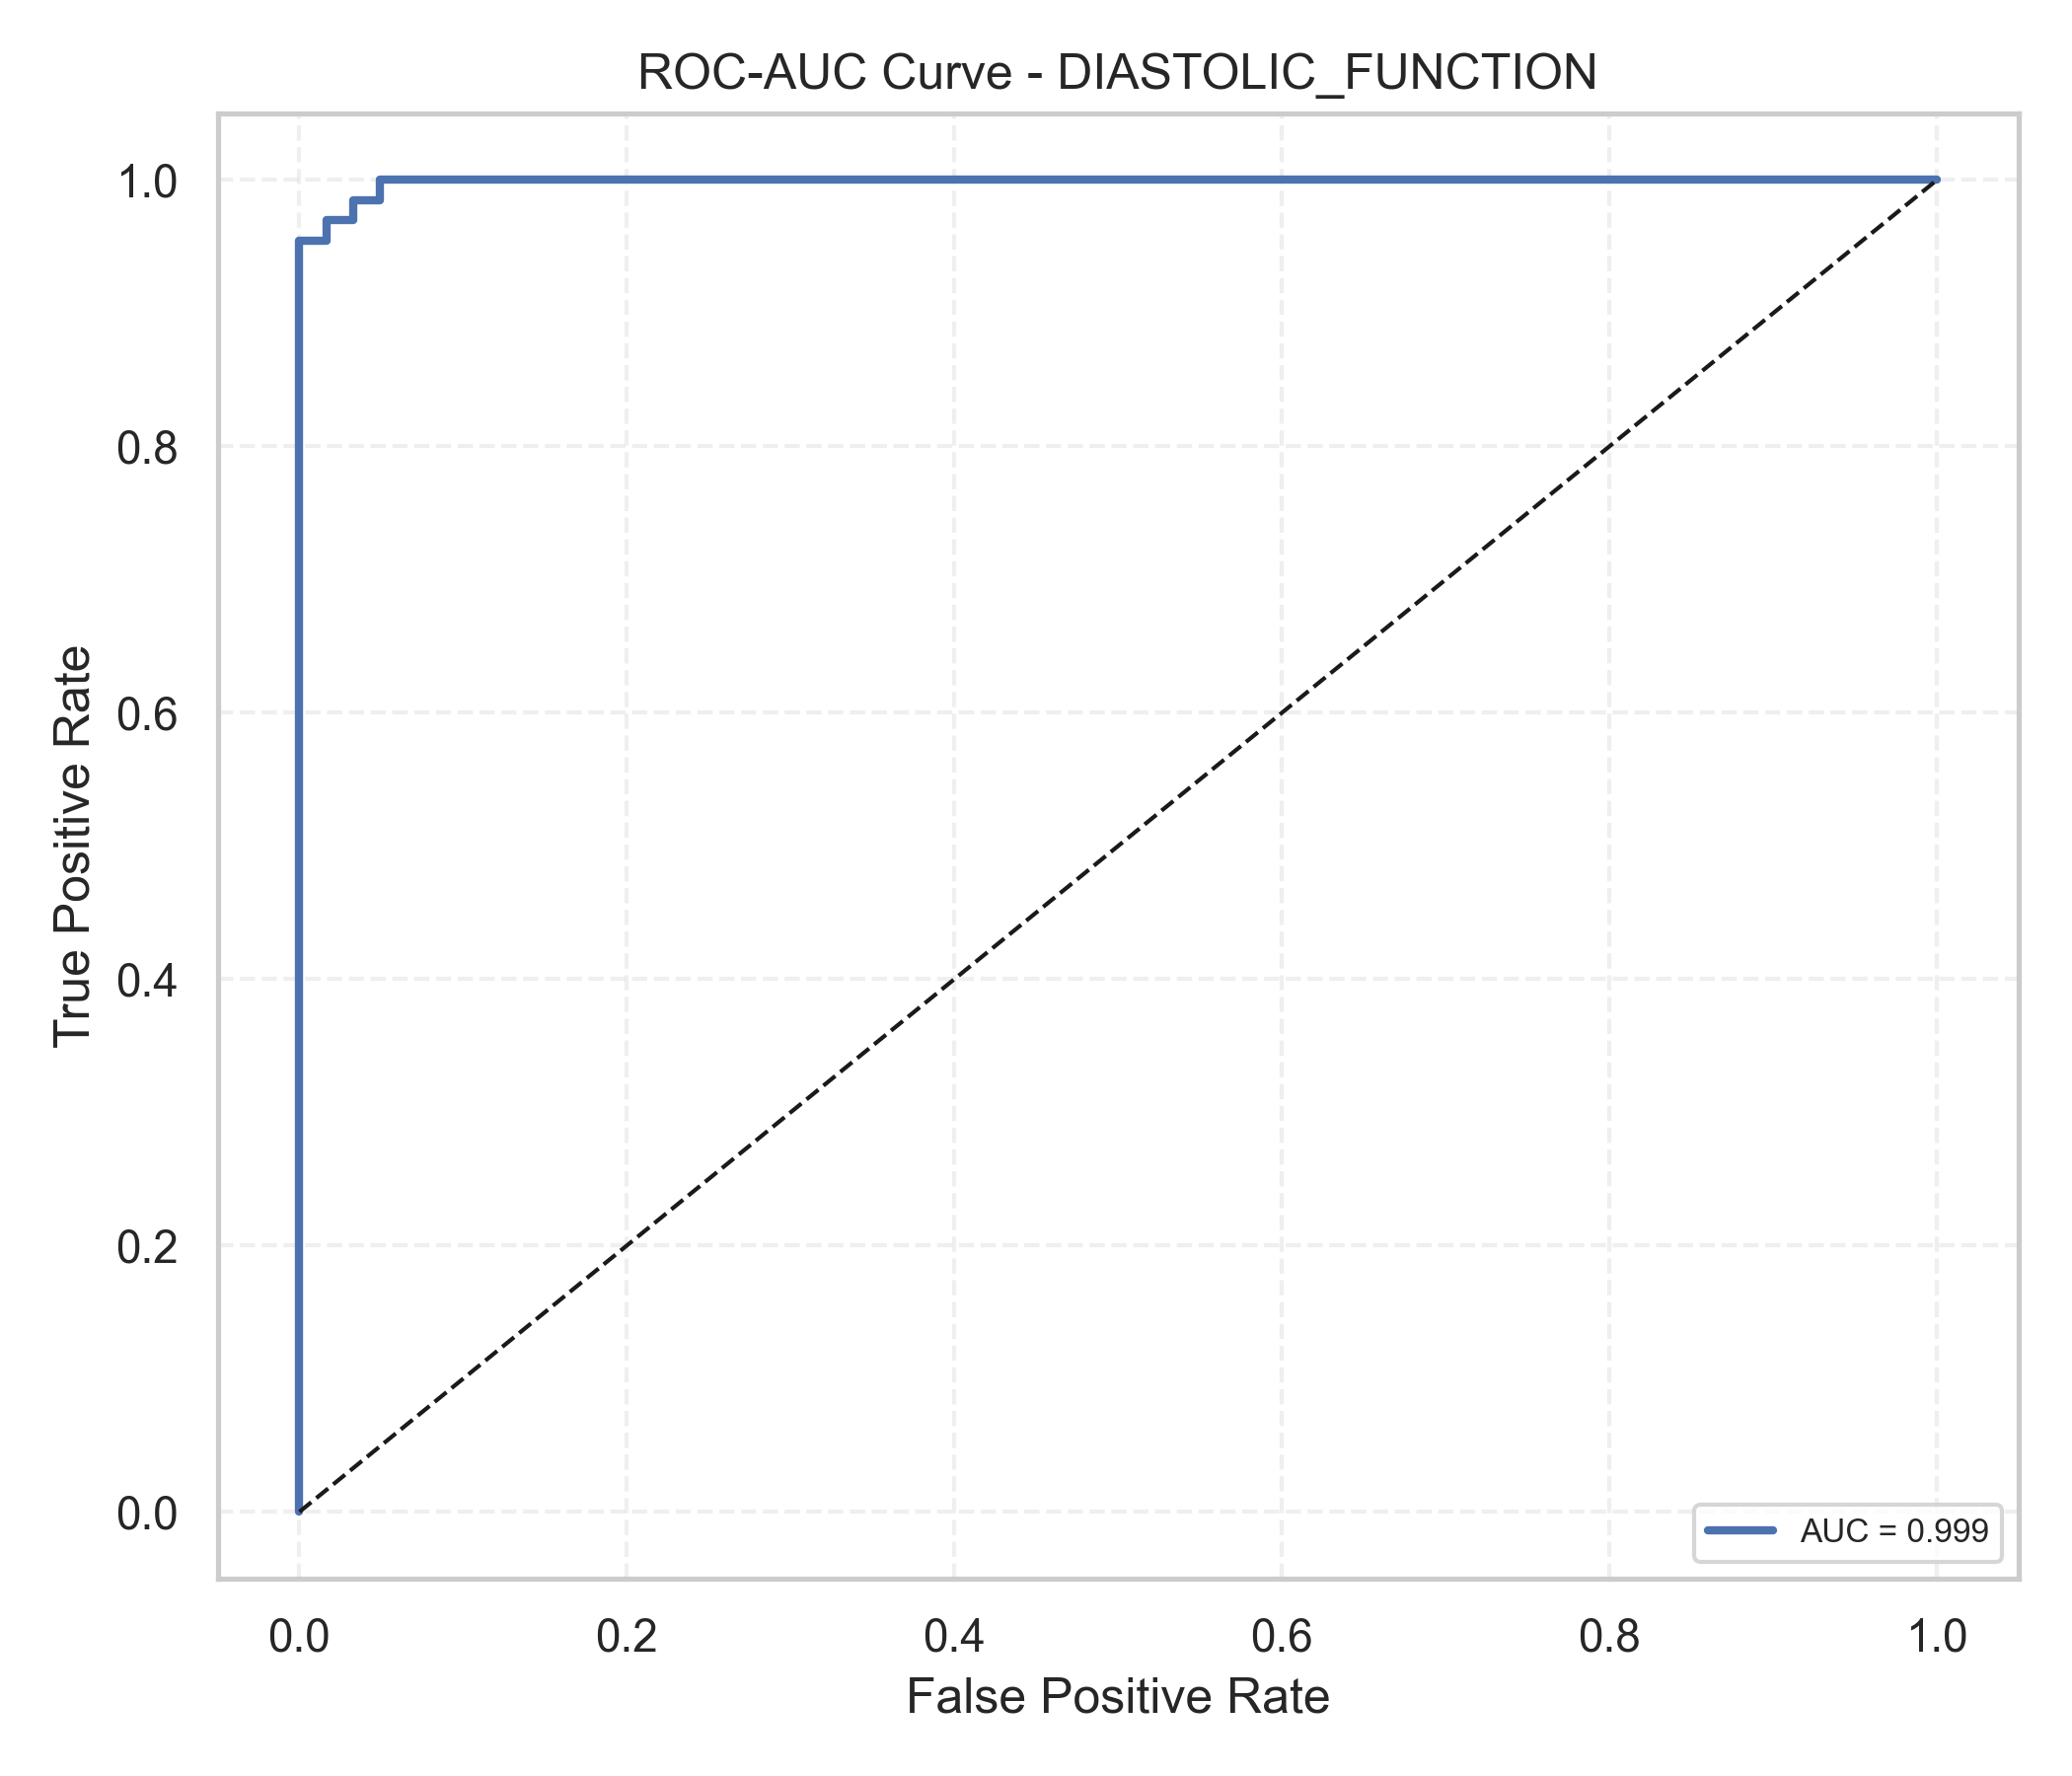
\includegraphics[width=\textwidth]{../../outputs/paper_plots/roc_auc_DIASTOLIC_FUNCTION.png}
\caption{DIASTOLIC\_FN}
\end{subfigure}
\caption{ROC-AUC curves for all five prediction categories (expanded benchmark).}
\label{fig:roc}
\end{figure*}

\section{Explainability, Robustness, and Calibration}

\subsection{Explainability}
The system supports:
\begin{enumerate}
\item SHAP global bar/summary importance.
\item SHAP local waterfall traces.
\item SHAP dependence plots.
\item PDP/ICE behavior curves.
\end{enumerate}

Integration with clinical workflows is facilitated through web-based interactive visualizations in the deployed React frontend.

\begin{figure*}[t]
\centering
\begin{subfigure}[b]{0.32\textwidth}
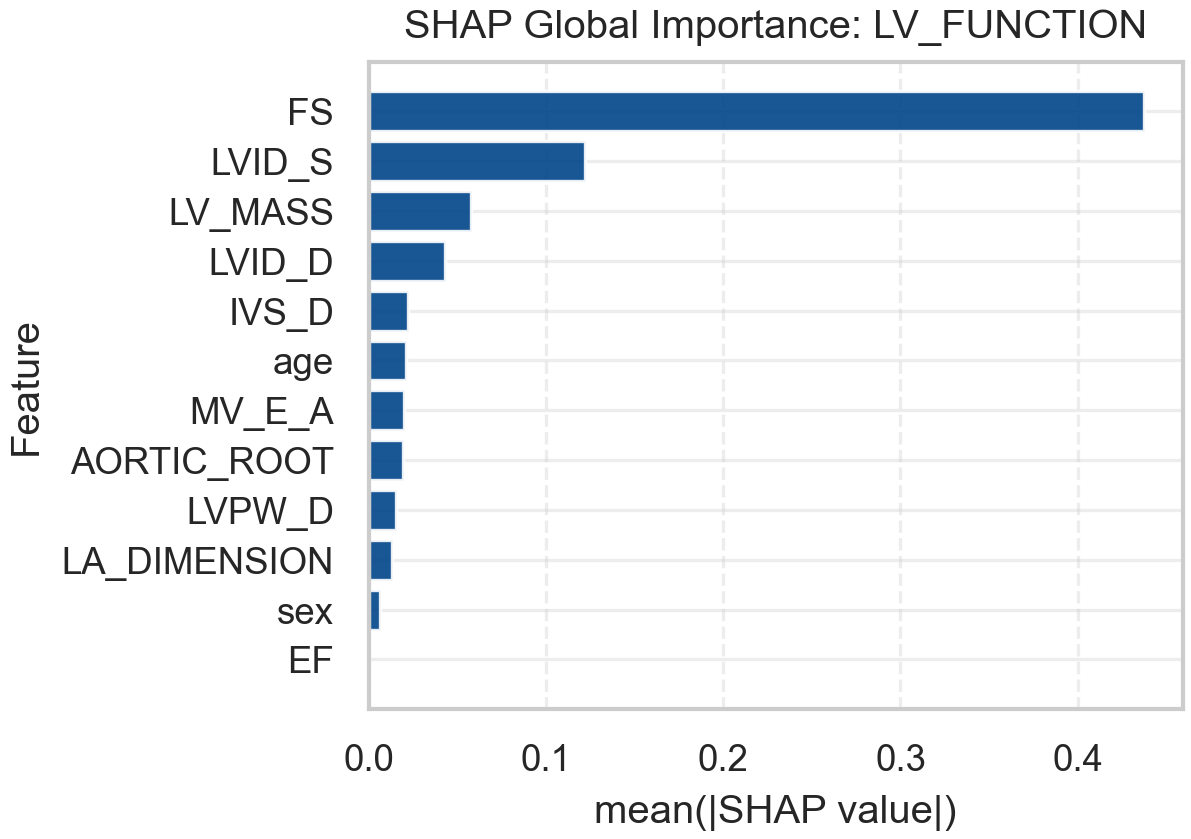
\includegraphics[width=\textwidth]{../../outputs/paper_plots/ieee_explainability/shap_global_bar_LV_FUNCTION.png}
\caption{SHAP global feature importance}
\end{subfigure}
\begin{subfigure}[b]{0.32\textwidth}
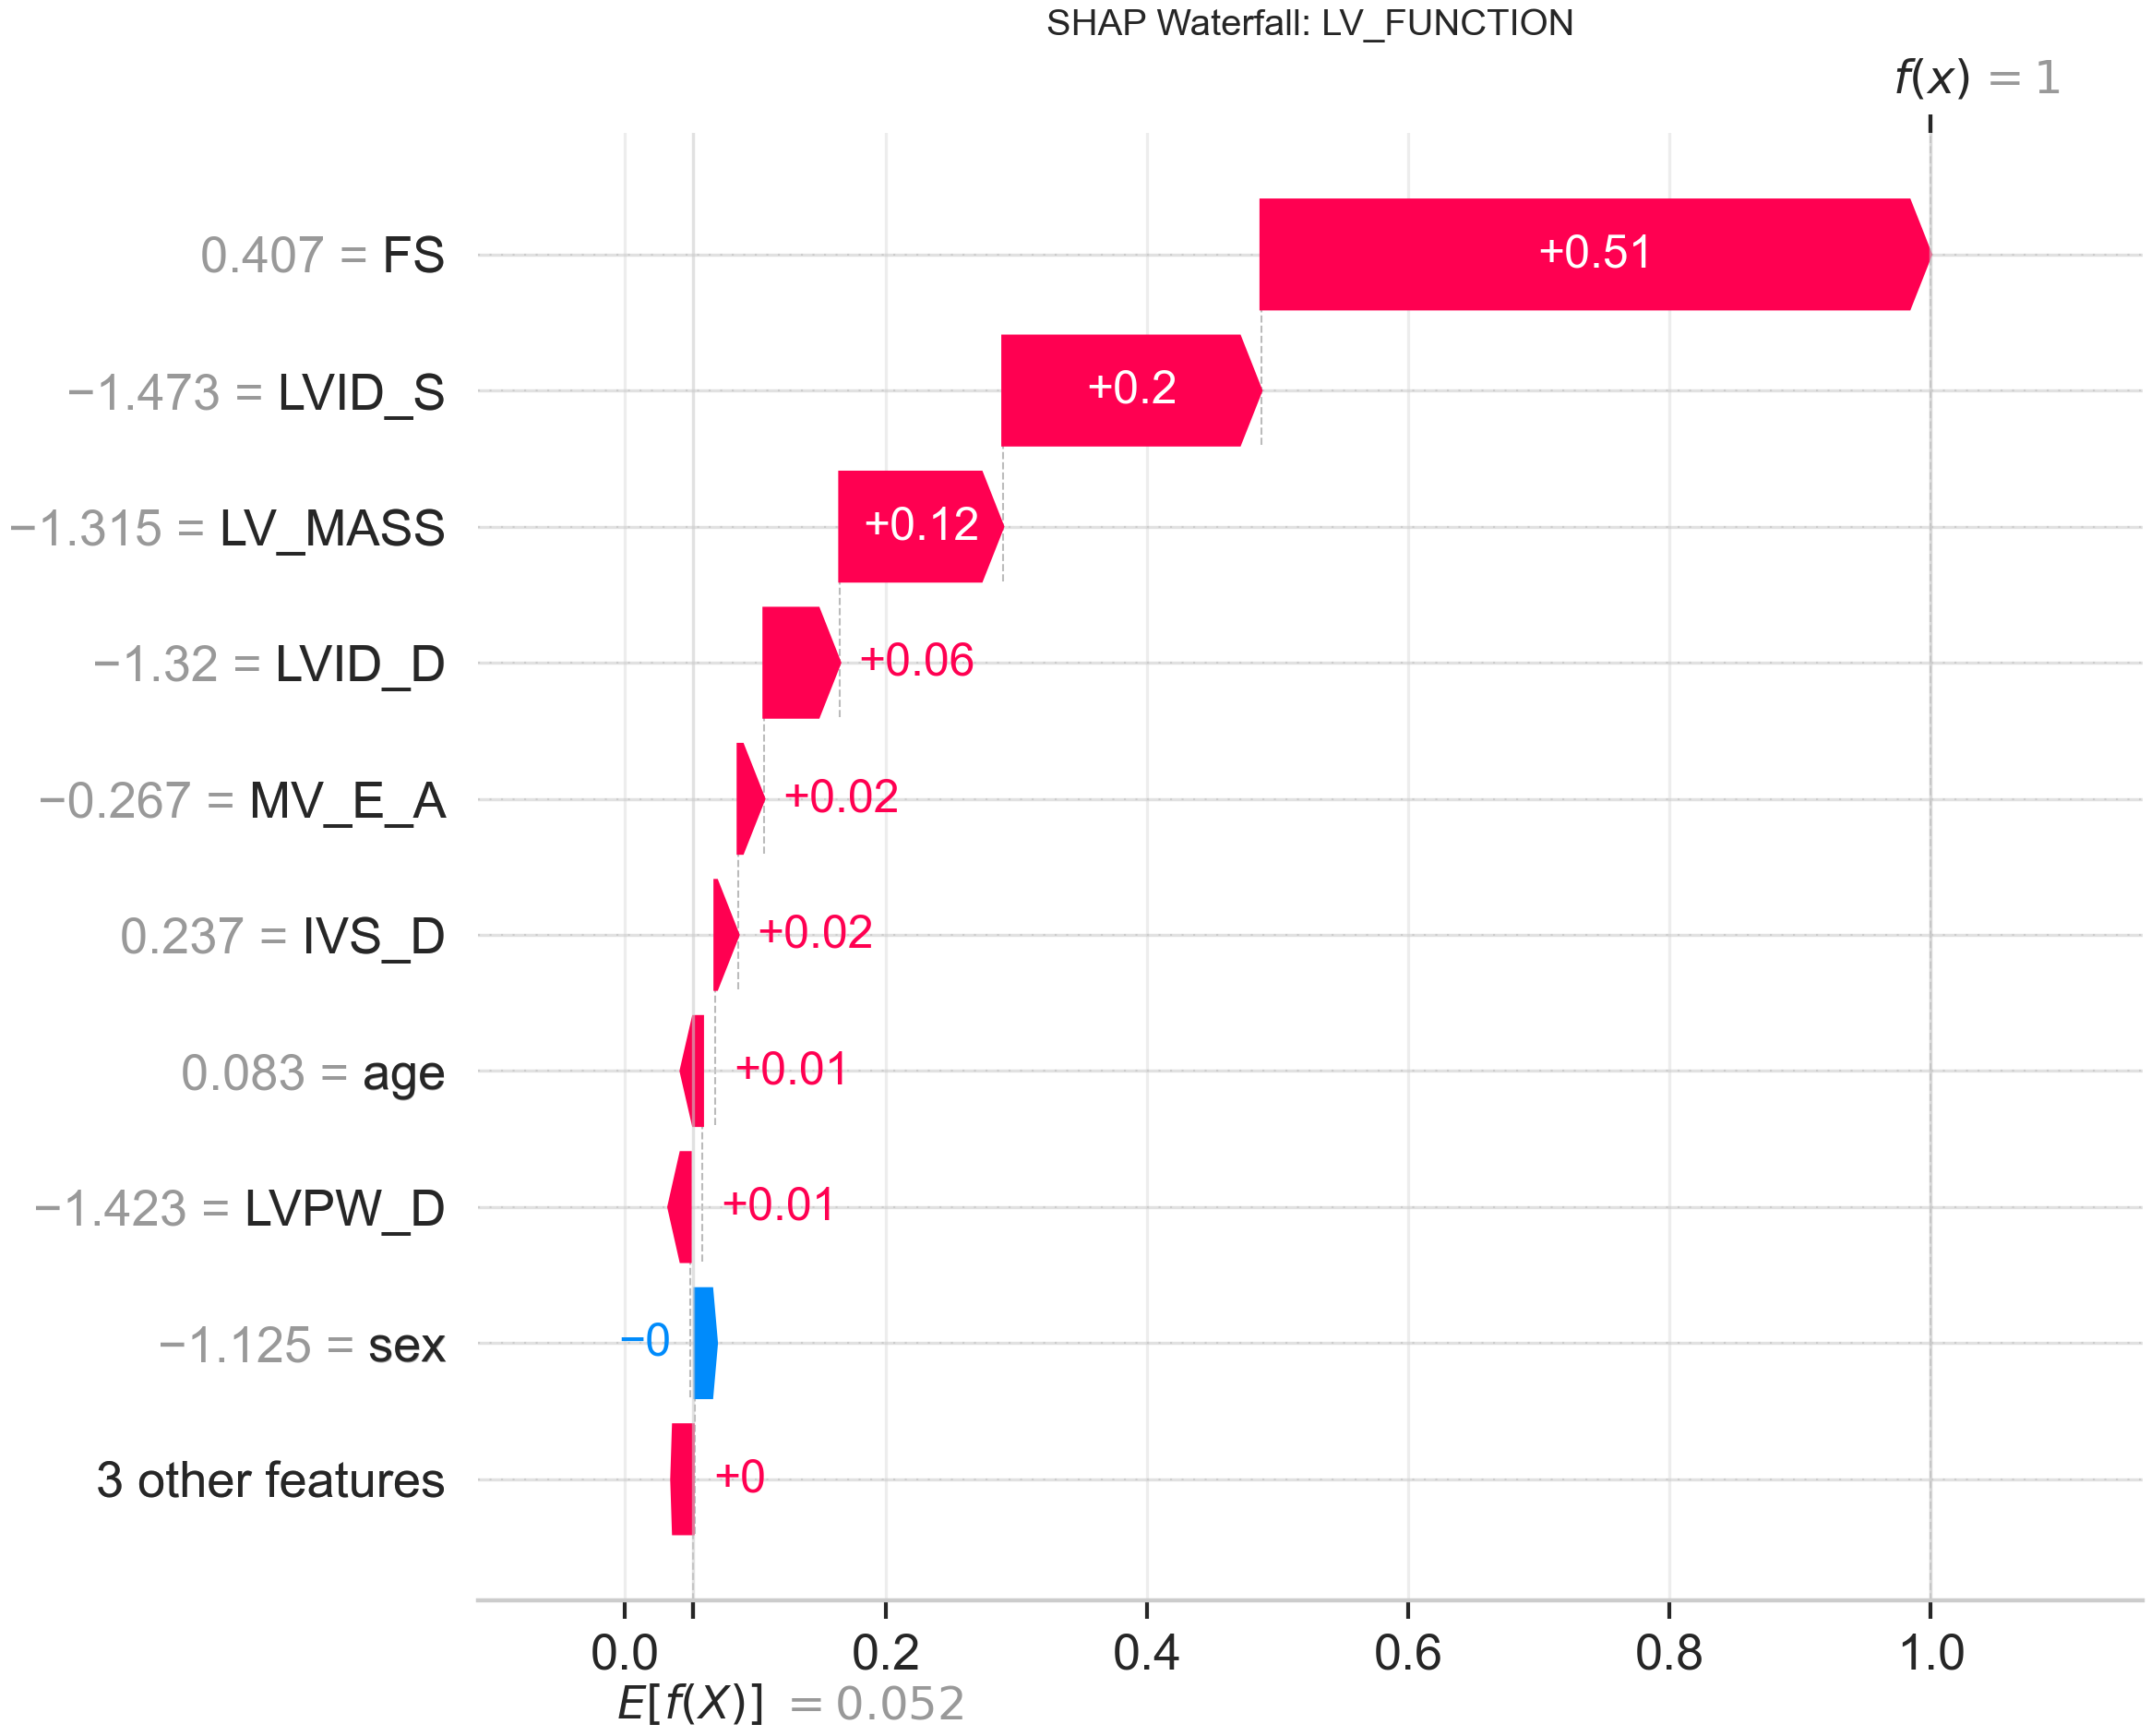
\includegraphics[width=\textwidth]{../../outputs/paper_plots/ieee_explainability/shap_waterfall_LV_FUNCTION.png}
\caption{SHAP local waterfall (example case)}
\end{subfigure}
\begin{subfigure}[b]{0.32\textwidth}
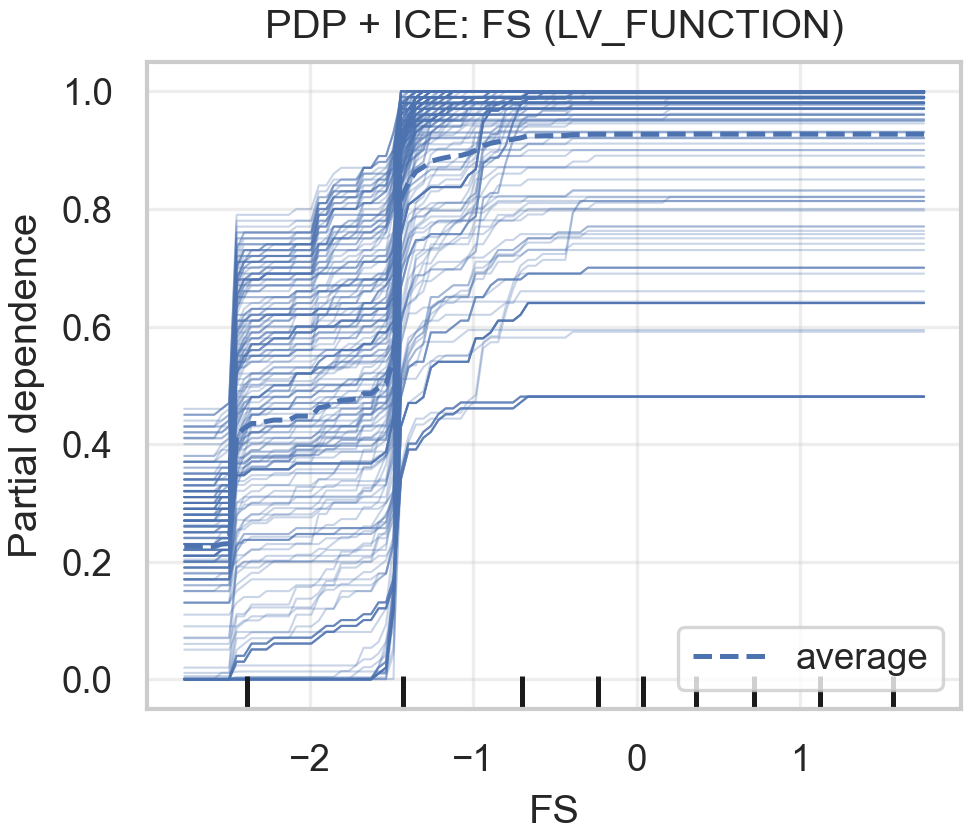
\includegraphics[width=\textwidth]{../../outputs/paper_plots/ieee_explainability/pdp_ice_LV_FUNCTION_FS.png}
\caption{PDP/ICE for FS feature}
\end{subfigure}
\caption{Explainability analyses: SHAP and PDP/ICE visualizations for LV\_FUNCTION category.}
\label{fig:explainability}
\end{figure*}

\subsection{Sensitivity and Uncertainty}
Implemented analyses include:
\begin{enumerate}
\item One-at-a-time perturbation sensitivity.
\item Monte Carlo measurement noise propagation.
\item Global sensitivity summaries.
\end{enumerate}

\begin{figure*}[t]
\centering
\begin{subfigure}[b]{0.32\textwidth}
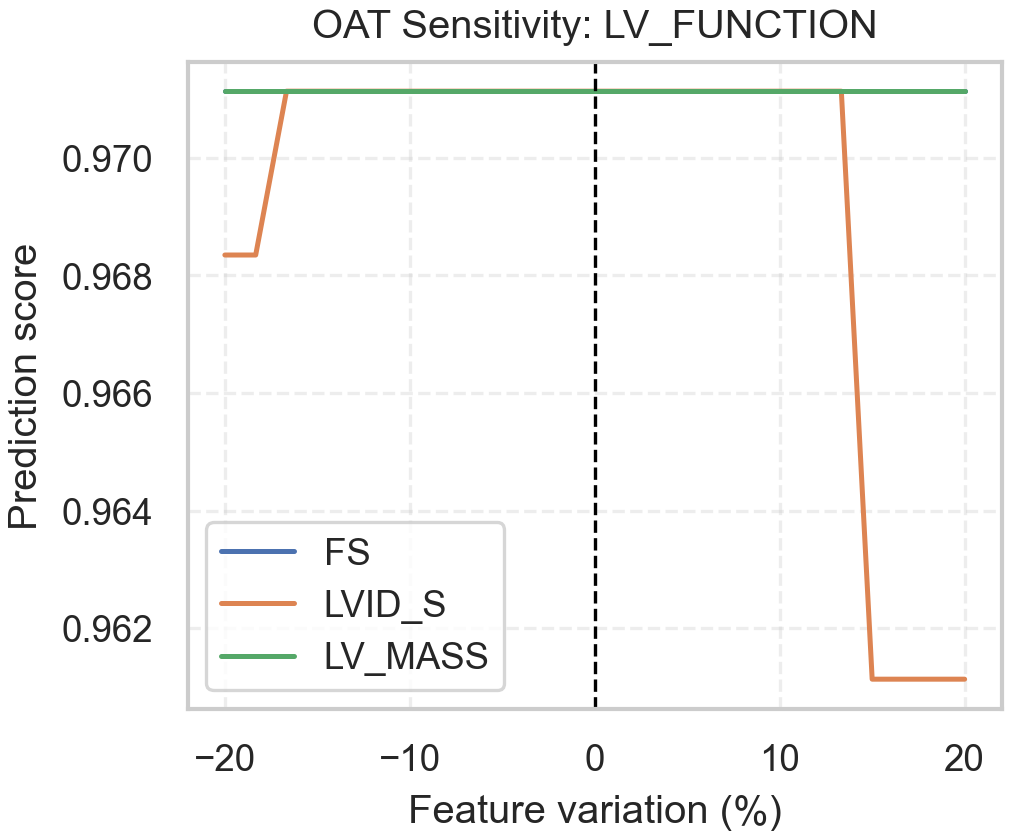
\includegraphics[width=\textwidth]{../../outputs/paper_plots/ieee_explainability/oat_sensitivity_LV_FUNCTION.png}
\caption{One-at-a-time sensitivity}
\end{subfigure}
\begin{subfigure}[b]{0.32\textwidth}
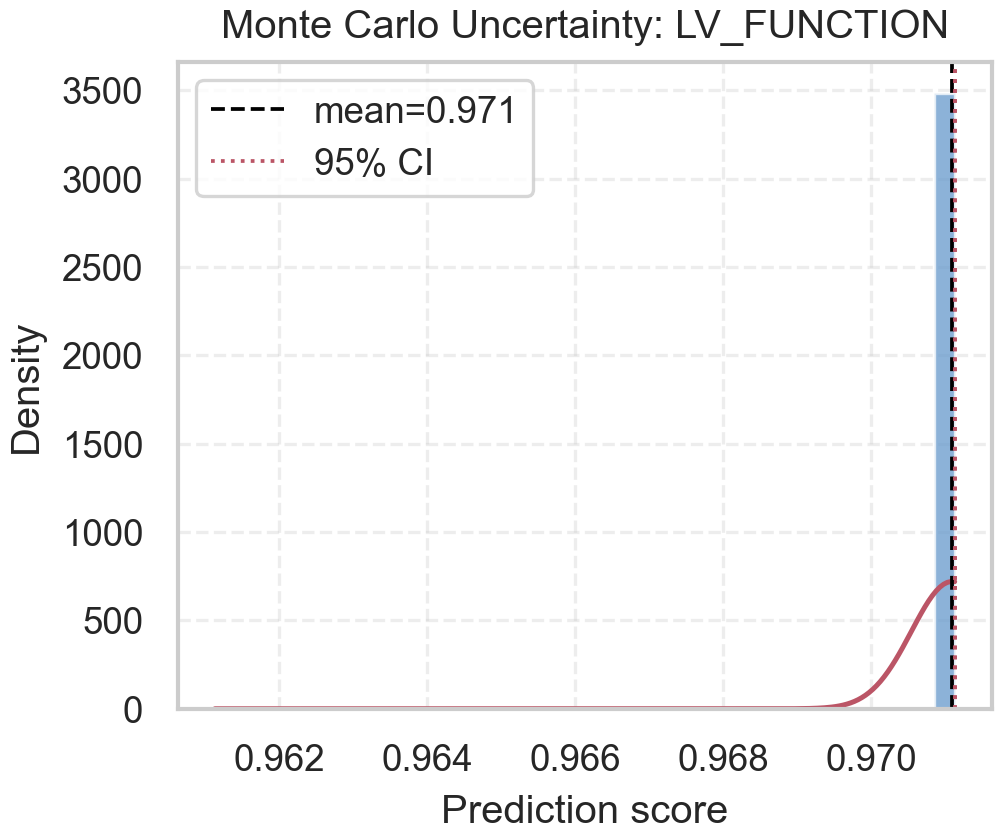
\includegraphics[width=\textwidth]{../../outputs/paper_plots/ieee_explainability/monte_carlo_LV_FUNCTION.png}
\caption{Monte Carlo noise propagation}
\end{subfigure}
\begin{subfigure}[b]{0.32\textwidth}
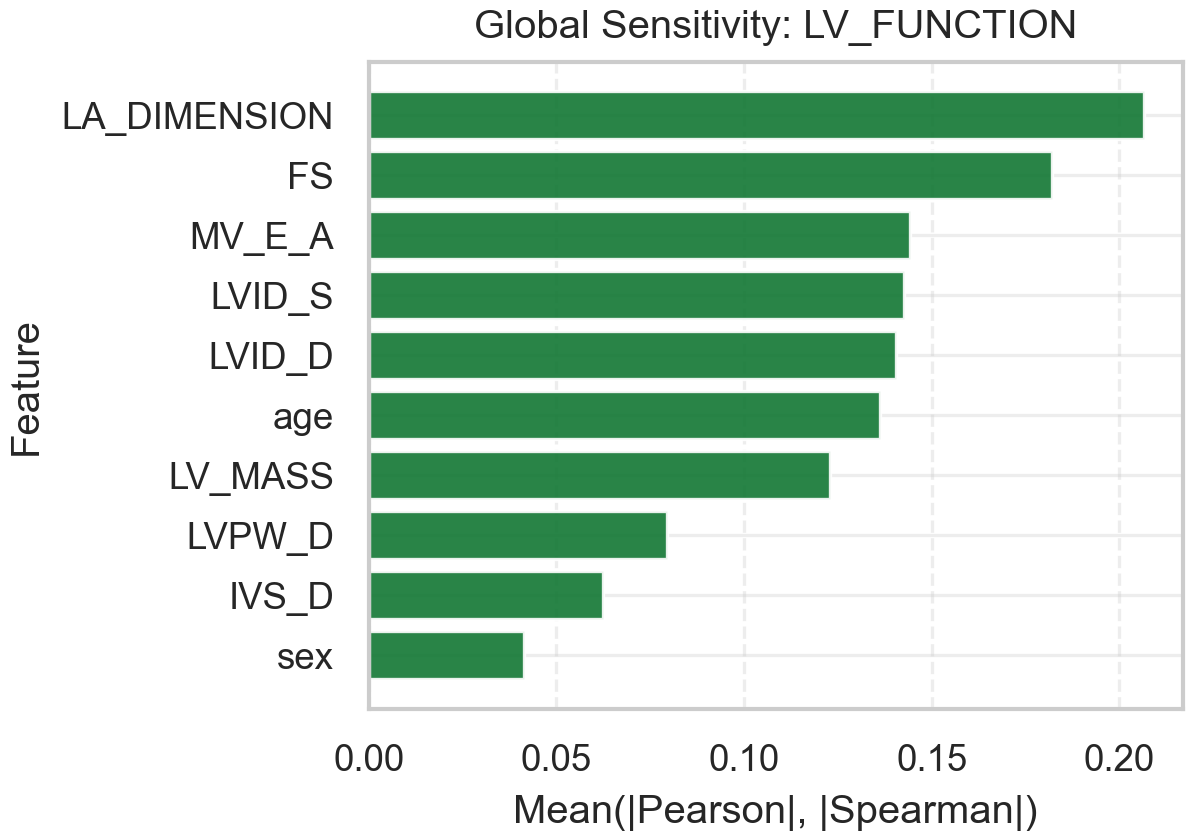
\includegraphics[width=\textwidth]{../../outputs/paper_plots/ieee_explainability/global_sensitivity_LV_FUNCTION.png}
\caption{Global sensitivity indices}
\end{subfigure}
\caption{Robustness and sensitivity analyses: perturbation, noise propagation, and global sensitivity for LV\_FUNCTION.}
\label{fig:robustness}
\end{figure*}

\subsection{Calibration}
Calibration is evaluated using reliability curves and Brier score formulation (Eq.~\ref{eq:brierscore}). Reliability visualizations are included per category in the supplementary figure set.



\section{Discussion}
This work is best interpreted as an end-to-end explainable clinical decision support system rather than only a classifier benchmark. The strongest practical value is integration completeness: extraction, interpretation, explainability, robustness, and deployment in one reproducible pipeline.

Clinical validation by expert cardiologists is future work, and would be essential for any real-world translational deployment.

The hybrid architecture ensures that deterministic rule-based outputs remain available for interpretability and safety assurance even if the ML component fails or produces low-confidence predictions.

\section{Ethics and Clinical Use}
\begin{enumerate}
\item De-identification is required before model-development usage.
\item Shared artifacts must not contain personally identifiable information.
\item The system is intended for decision support only and not autonomous diagnosis.
\item All clinical deployment requires institutional review board (IRB) approval and clinical validation studies.
\end{enumerate}

\section{Reproducibility}
Reproduction commands:
\begin{enumerate}
\item \texttt{python prepare\_training\_data.py}
\item \texttt{python train\_interpretation\_model.py}
\item \texttt{python generate\_fair\_model\_selection\_report.py}
\item \texttt{python compare\_models.py}
\item \texttt{python generate\_paper\_plots.py}
\item \texttt{python generate\_ieee\_explainability\_plots.py}
\end{enumerate}

Core package versions (from requirements.txt):
\begin{enumerate}
\item pandas $\geq$ 1.3.0
\item numpy $\geq$ 1.21.0
\item scikit-learn $\geq$ 1.0.0
\item shap $\geq$ 0.41.0
\item scipy $\geq$ 1.7.0
\item flask $\geq$ 2.0.0
\end{enumerate}

Fixed seed value: 42 (used throughout all experiments for reproducibility).

\section{Conclusion}
The proposed framework provides a submission-ready example of an end-to-end explainable clinical decision support pipeline for echocardiography report interpretation. Under fair repeated cross-validation benchmarking, Gradient Boosting is the strongest baseline among compared classical models, and on fixed-test expanded evaluation the system reaches 0.981 average accuracy and 0.978 macro F1 across five categories. The hybrid rule-ML design enables strong predictive performance with operational safety fallback and transparent interpretation pathways suitable for translational deployment studies.

Future work includes clinical validation studies, integration with hospital PACS/EHR systems, and extension to video-based analysis for real-time assessment in the echocardiography suite.

\begin{thebibliography}{99}

\bibitem{madani2018}
A. Madani, M. Arnaout, M. Mofrad, and R. Arnaout, ``Fast and accurate view classification of echocardiograms using deep learning,'' \textit{npj Digital Medicine}, vol. 1, no. 6, 2018.

\bibitem{ouyang2020}
D. Ouyang \textit{et al}., ``Video-based AI for beat-to-beat assessment of cardiac function,'' \textit{Nature}, vol. 580, pp. 252--256, 2020.

\bibitem{bernard2018}
O. Bernard \textit{et al}., ``Deep learning techniques for automatic MRI cardiac multi-structures segmentation and diagnosis: is the problem solved?'' \textit{IEEE Transactions on Medical Imaging}, vol. 37, no. 11, pp. 2514--2525, 2018.

\bibitem{lundberg2017}
S. M. Lundberg and S.-I. Lee, ``A unified approach to interpreting model predictions,'' in \textit{Advances in Neural Information Processing Systems}, vol. 30, 2017.

\bibitem{holzinger2019}
A. Holzinger \textit{et al}., ``Causability and explainability of artificial intelligence in medicine,'' \textit{Wiley Interdisciplinary Reviews: Data Mining and Knowledge Discovery}, vol. 9, no. 4, 2019.

\bibitem{fawcett2006}
T. Fawcett, ``An introduction to ROC analysis,'' \textit{Pattern Recognition Letters}, vol. 27, no. 8, pp. 861--874, 2006.

\bibitem{chicco2020}
D. Chicco and G. Jurman, ``The advantages of the Matthews correlation coefficient over F1 score and accuracy in binary classification evaluation,'' \textit{BMC Genomics}, vol. 21, no. 6, 2020.

\bibitem{friedman2001}
J. H. Friedman, ``Greedy function approximation: A gradient boosting machine,'' \textit{The Annals of Statistics}, vol. 29, no. 5, pp. 1189--1232, 2001.

\bibitem{hastie2009}
T. Hastie, R. Tibshirani, and J. Friedman, \textit{The Elements of Statistical Learning}, 2nd ed. New York, NY, USA: Springer, 2009.

\bibitem{pedregosa2011}
F. Pedregosa \textit{et al}., ``Scikit-learn: Machine learning in Python,'' \textit{Journal of Machine Learning Research}, vol. 12, pp. 2825--2830, 2011.

\bibitem{ribeiro2016}
M. T. Ribeiro, S. Singh, and C. Guestrin, ``Why should I trust you? Explaining the predictions of any classifier,'' in \textit{Proceedings of ACM SIGKDD}, 2016, pp. 1135--1144.

\bibitem{molnar2022}
C. Molnar, \textit{Interpretable Machine Learning}, 2nd ed., 2022.

\end{thebibliography}

\end{document}
